\startchapter{Empirical Evidence}
\label{chapter:Exp}

In this chapter, we are going to report our result from a empirical evidence. We use 5 macroeconomic variables to predict GDP for Canada. 

\section{Why we choose financial data?}

\subsection{Financial data available and helpful}

\citeA{Andreou2013a} demonstrate that daily financial data can help forecast and nowcast the quarterly GDP growth. (Need to fix)  \citeA{BANBURA2014} show  real time daily financial data can better the nowcasting of low frequency macroeconomic data.  \citeA{Chauvet2014}  and  \citeA{Ferrara2013}  have recently shown that  daily financial series have a significant forecasting power when it comes to the US growth, specially when the volatility of those signals is considered as a explaining factor and not only its returns. 


We choose gross domestic product(GDP) for Canada as target variable. GDP is a very important indicator for economic activity and has been used for economic decision and public policy analysis in many institution. Forecasting GDP is very challenging since it is related to and affect many macroeconomic factors such as employment, consumption, and  export. In this chapter, we are going to show BSTS-U-MIDAS can help us to extract signal in high frequency data to improve forecast accuracy. In practice, ARIMA modle such as AR(1) and AR(4) perform very well, and a few model can outperform them \cite{Koopman2013}. Our empirical evidence shows that BSTS-U-MIDAS model performs very well during the 2007-2011 financial crisis period. It shows BSTS-U-MIDAS model is more capable to predict the change points and structural breaks.     


  




\section{Data}

We choose 5 macroeconomic variables in regression component of our model. They are daily GST stock market index and West Texas crude oil prices, monthly unemployment rate, spread between 10 years and 3 month government bonds interest rate, and  housing start data. Those variable are high correlated to Canadian GDP. (Detail of the data is discussed in Appendix B)

The data of Real GDP for Canada and housing start is taken from Statistic Canada. The data of monthly unemployment rate,  spread between 10 years and 3 month government bonds interest rate, and   West Texas crude oil prices are taken from FRED® database. Toronto Stock Exchange (TSX) composite index is taken from Yahoo finance. 

We estimate three models with different sets of data. First model has  monthly unemployment rate, spread between 10 years and 3 month government bonds interest rate, and Toronto Stock Exchange (TSX) composite index. Second model has housing start and the data in first model. Third model has West Texas crude oil prices and the data in second model. In this section we are going to discuss the detail for third model and some remarkable difference between three models. (See the details for first and second model  in Appendix C.)  




\subsection{Target: GDP growth rate for Canada}

Our target variable is total gross domestic product for Canada. It is a quarterly ,seasonal adjusted data which measured by expenditure in constant prices. Figure ~\ref{fig:gdp-growth} shows the dynamics of GDP for Canada between 1980 to 2015.


\begin{figure}[h]
\centering
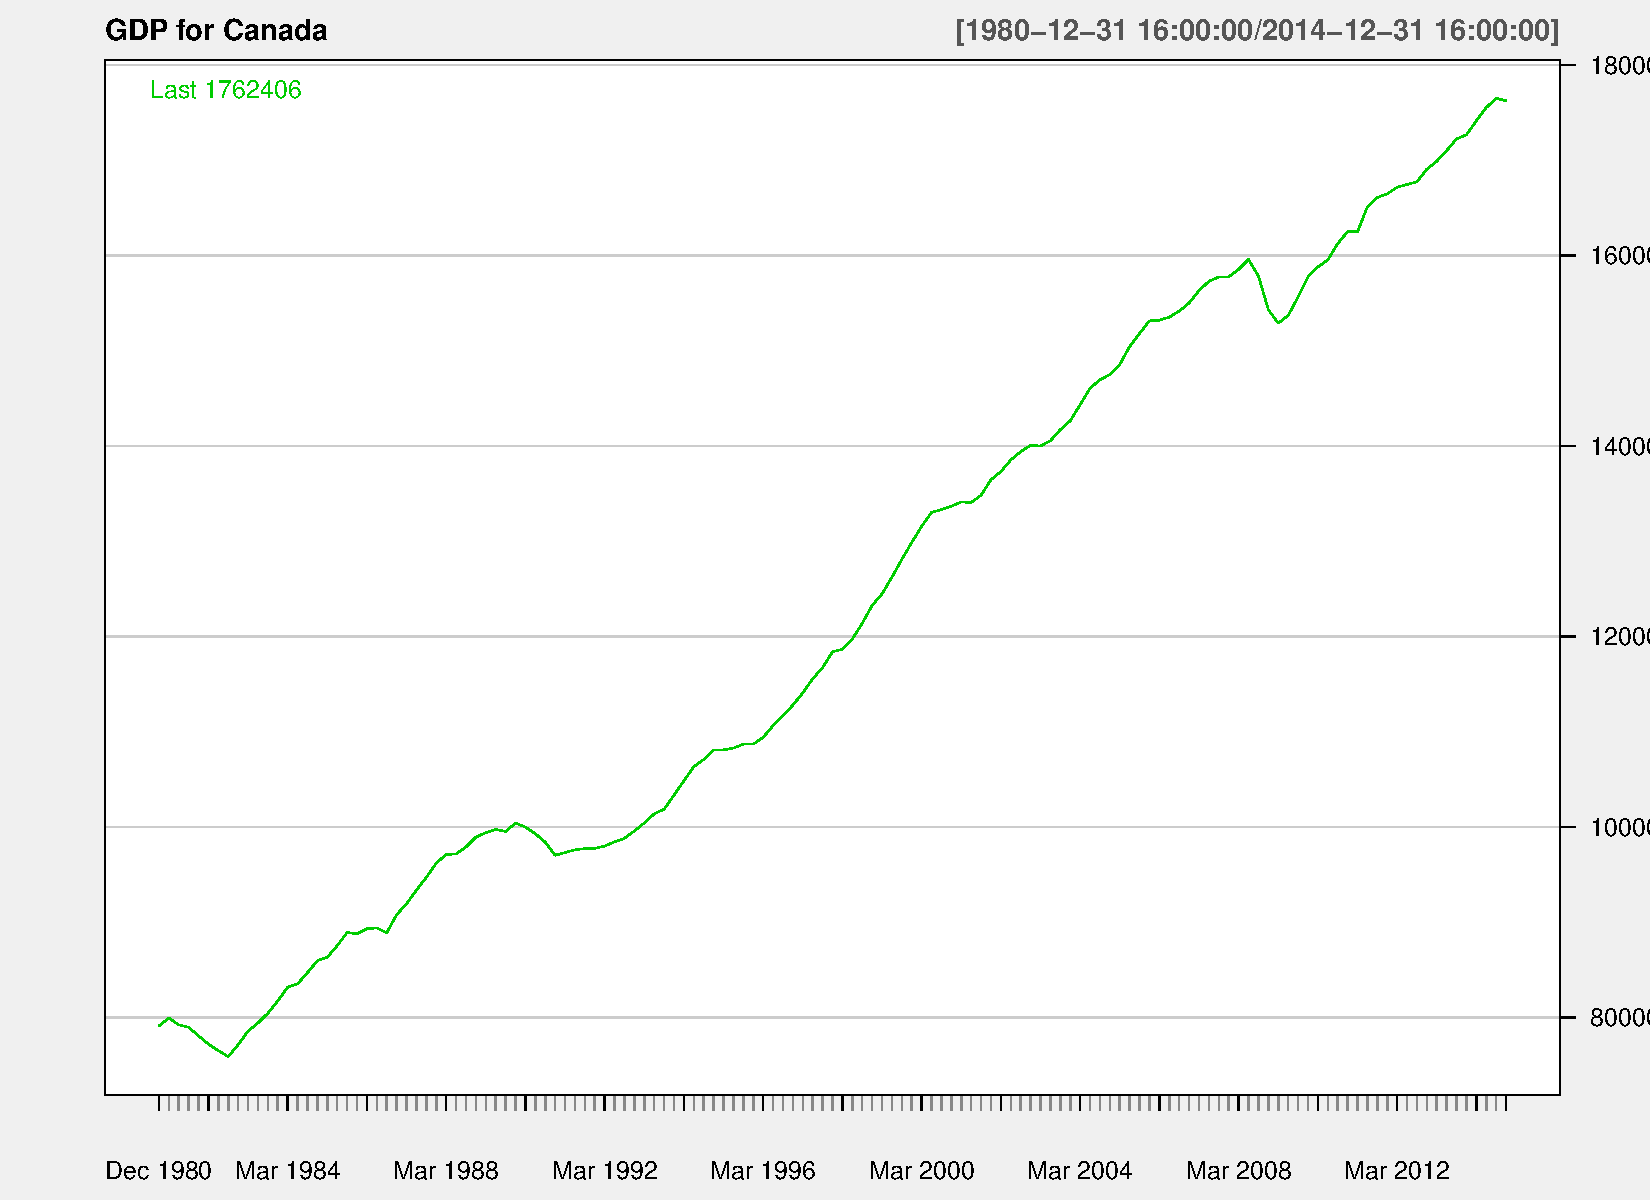
\includegraphics[width=0.6\linewidth]{Figures/gdp-report}
\caption{Total Gross Domestic Product for Canada 1980/07-2015/01 Quarterly}
\label{fig:gdp-report}
\end{figure}



In order to compare performance of BSTS, ARIMA and Boosting models, we need a stationary time series data for the ARIMA, so we calculate the log differenced GDP as target variable in all three models. 

\begin{figure}[h]
	\centering
	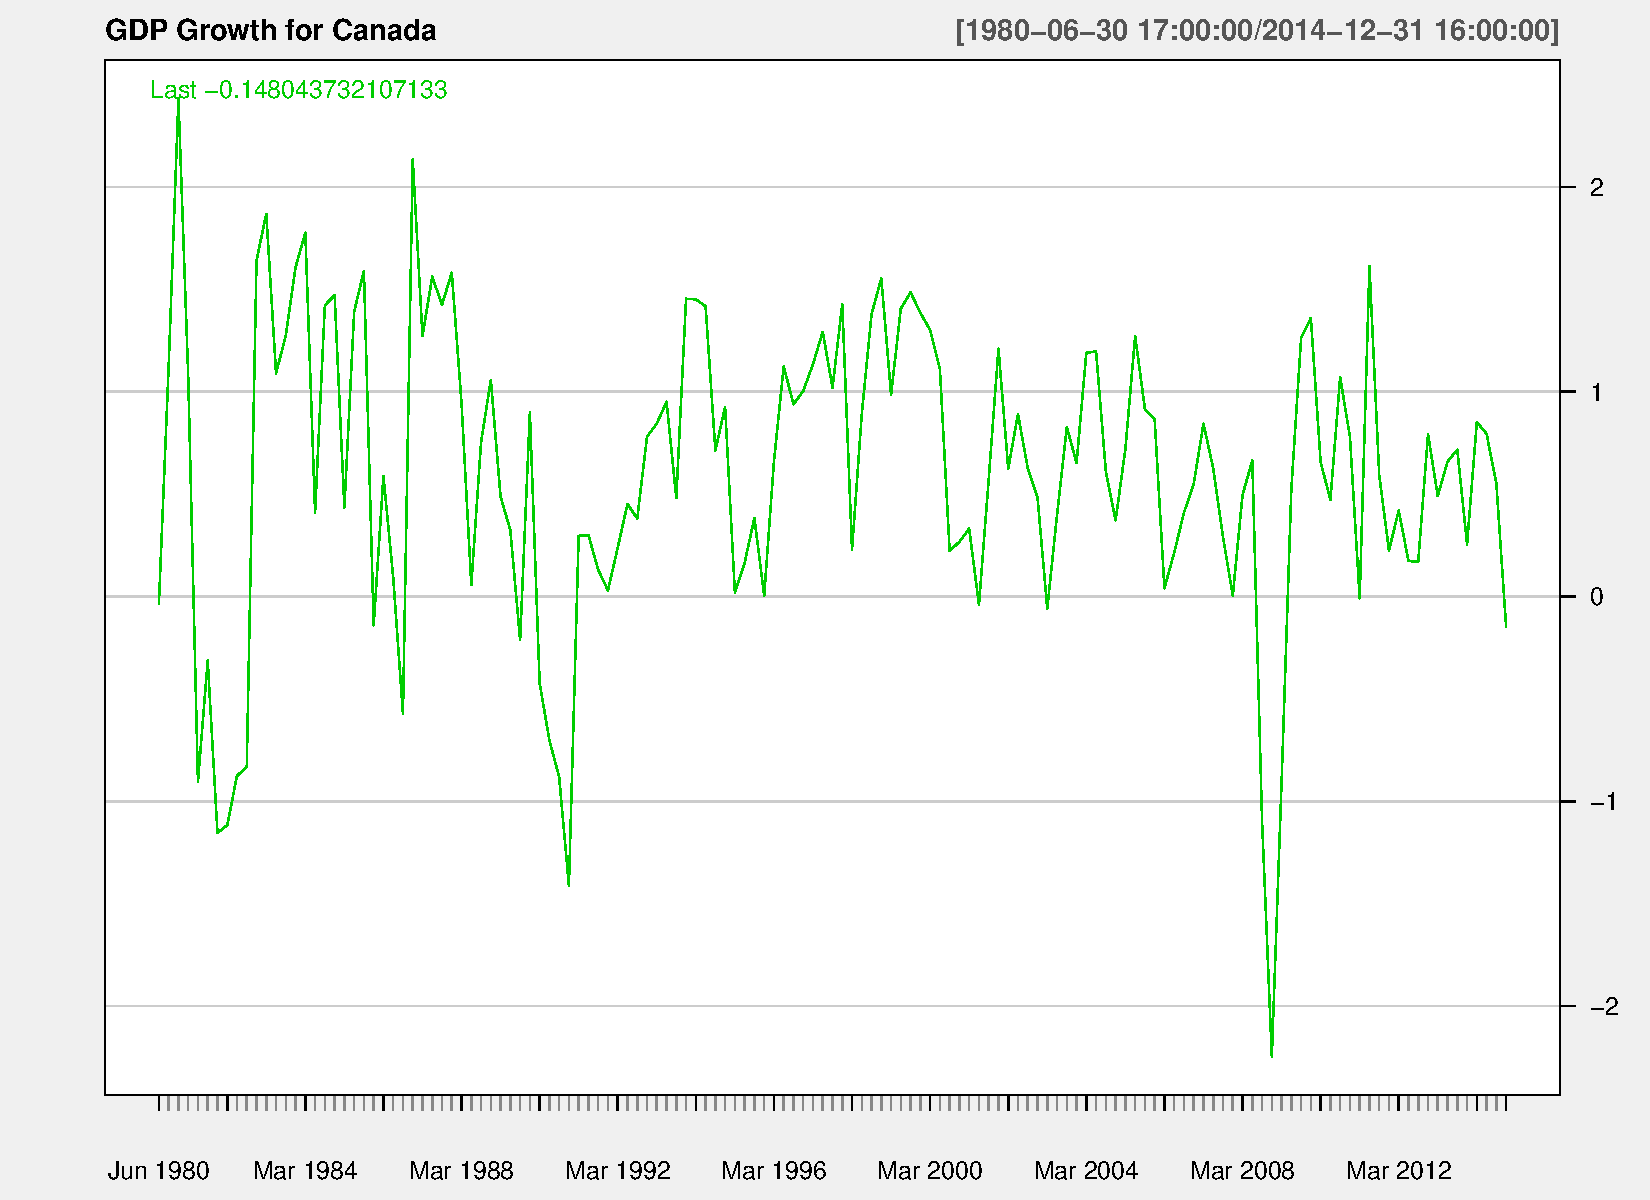
\includegraphics[width=0.6\linewidth]{Figures/gdp-growth-report}
	\caption{Gross Domestic Product Growth Rate for Canada 1980/07-2015/01 Quarterly}
	\label{fig:gdp-growth}
\end{figure}


For all predictors, we also include heads and lags in the regression. For a monthly data, we keep 23 month lags (two years). For a daily data, we keep 12*22-1 lags (one year). Then in first model, the number of total predictors (explanatory variables) in the regression component is 313, but we only have 139 observations. Our model is a fat regression type model.  With their lags of those variables, the design matrix in regression component become much fatter. Our BSTS-U-MIDAS model does not select some specific variables. Instead, 
it calculates the probability of inclusion of variables and predict the posterior distribution of the prediction. 



\subsection{Pre-process of the data: transformation and whitening}


As we mention, all predictors data are realigned to match up the quarterly frequency by skipping sampled method that we discuss in previous chapter. All predictors information please see appendix B. 

Due to the data availability, we match up all data at a window between 1986 fourth quarter to 2015 first quarter by using MIDAS (mixed frequency sampling) method in first and second models. The third model has the data at a window between 1986 fourth quarter to 2015 first quarter since we only have West Texas crude oil prices data down to 1986 fourth quarter. After a MIDAS skipping sampled transformation, each monthly time series data becomes matrix with 3 quarterly time series data components, and each daily time series data becomes matrix with 22*3 time series data components.

The date set is ragged. Different time series data has different most recent data point. For example, for the daily data such as TSX composite index, we choose the data up to May 28. Since the statistics Canada publishes the first quarter's GDP data on May 29, 2015, we are able to keep updating our forecasting practice using daily data until May 28, 2015. In terms of monthly data, we are able to include data up to March 2015.  


In order to avoid spurious regression, we detrend, deseasonalize, and scale the predictors using decomp command in R package "forecast". The target variable is seasonally adjusted. (In our case, deseasonalizing target variable improve the forecasting performance, so we choose to deseasonalize target variable. ) For daily data such as TSX index and oil price, we also take first order log difference to get stationarity, so in some sense, the return of TSX index and oil price are included in model. 

The rationale behind whitening is to avoid the spurious regression \cite{Scott2014}. Without the common trend and seasonality, the variation of target variable can be more accurately estimated by the variation of predictors. 



\section{Results: one period ahead forecasting / nowcasting}



In our practice, we use a generalized local trend model with AR(4) and regression model. (See Appendix C for detial). We add AR terms of target variable in the model since in order to utilize the information of lagged target variables for forecasting. For simplicity, we include AR terms up to AR(4) since our target variable is quarterly data. 


In our BSTS-U-MIDAS model, since we run a recursive algorithm, the filtered observation data is one period ahead forecas. It can be seen in a state space presentation of BSTS-U-MIDAS model, the expected filtered "observation" is estimated by the predicted state plus regression component:

Say $ GDP^t = (gdp_1, ..., gdp_t) $ be the vector of observation up to time t. The \textit{filtering} distributions, $p(\alpha_t|GDP^{t}) $ can be computed recursively as follows, $\alpha$ are the states which are needed to estimated in model:

First, we start with $ \alpha_0 \sim N(m_0, C_0) $ at time $0$, where $a_t$ include level $\mu_t$ and slope or drift $b_t$.

Then the one step forecast for the \textit{state} is
$$ \alpha_t|GDP^{t-1} \sim N(a_t, R_t) $$
where $a_t = G_t \cdot m_{t-1}$ , and $R_t = G_t C_{t-1} G_t^\prime + W_t$. In our BSTS model, transition or system matrix $G_t$ is $2 \times 2$ matrix. (The detail is discussed in Appendix A and C)  



\subsection{Distribution of one step ahead forecast for observations}

in MCMC iteration

One step forecast for the \textit{observation} can be estimated as follows: 
$$ gdp_t|GDP^{t-1}, X^{1:t-1}  \sim N(f_t, Q_t) $$
where $f_t = F_t \cdot a_t  + z_{t}$, and $Q_t = F_t R_{t-1} F_t^\prime + V_t$. $F_t$ is the observation matrix, and $z_{t} = \beta *  x_{t}$ is regression component, and  $X^{1:t-1}$ is the design matrix which includes all the covariates. $R_{t}$ is the covariance matrix for state $\alpha_{t}$, and $V_t$ is the covariance matrix for observation error.


\begin{figure}[h]
\centering
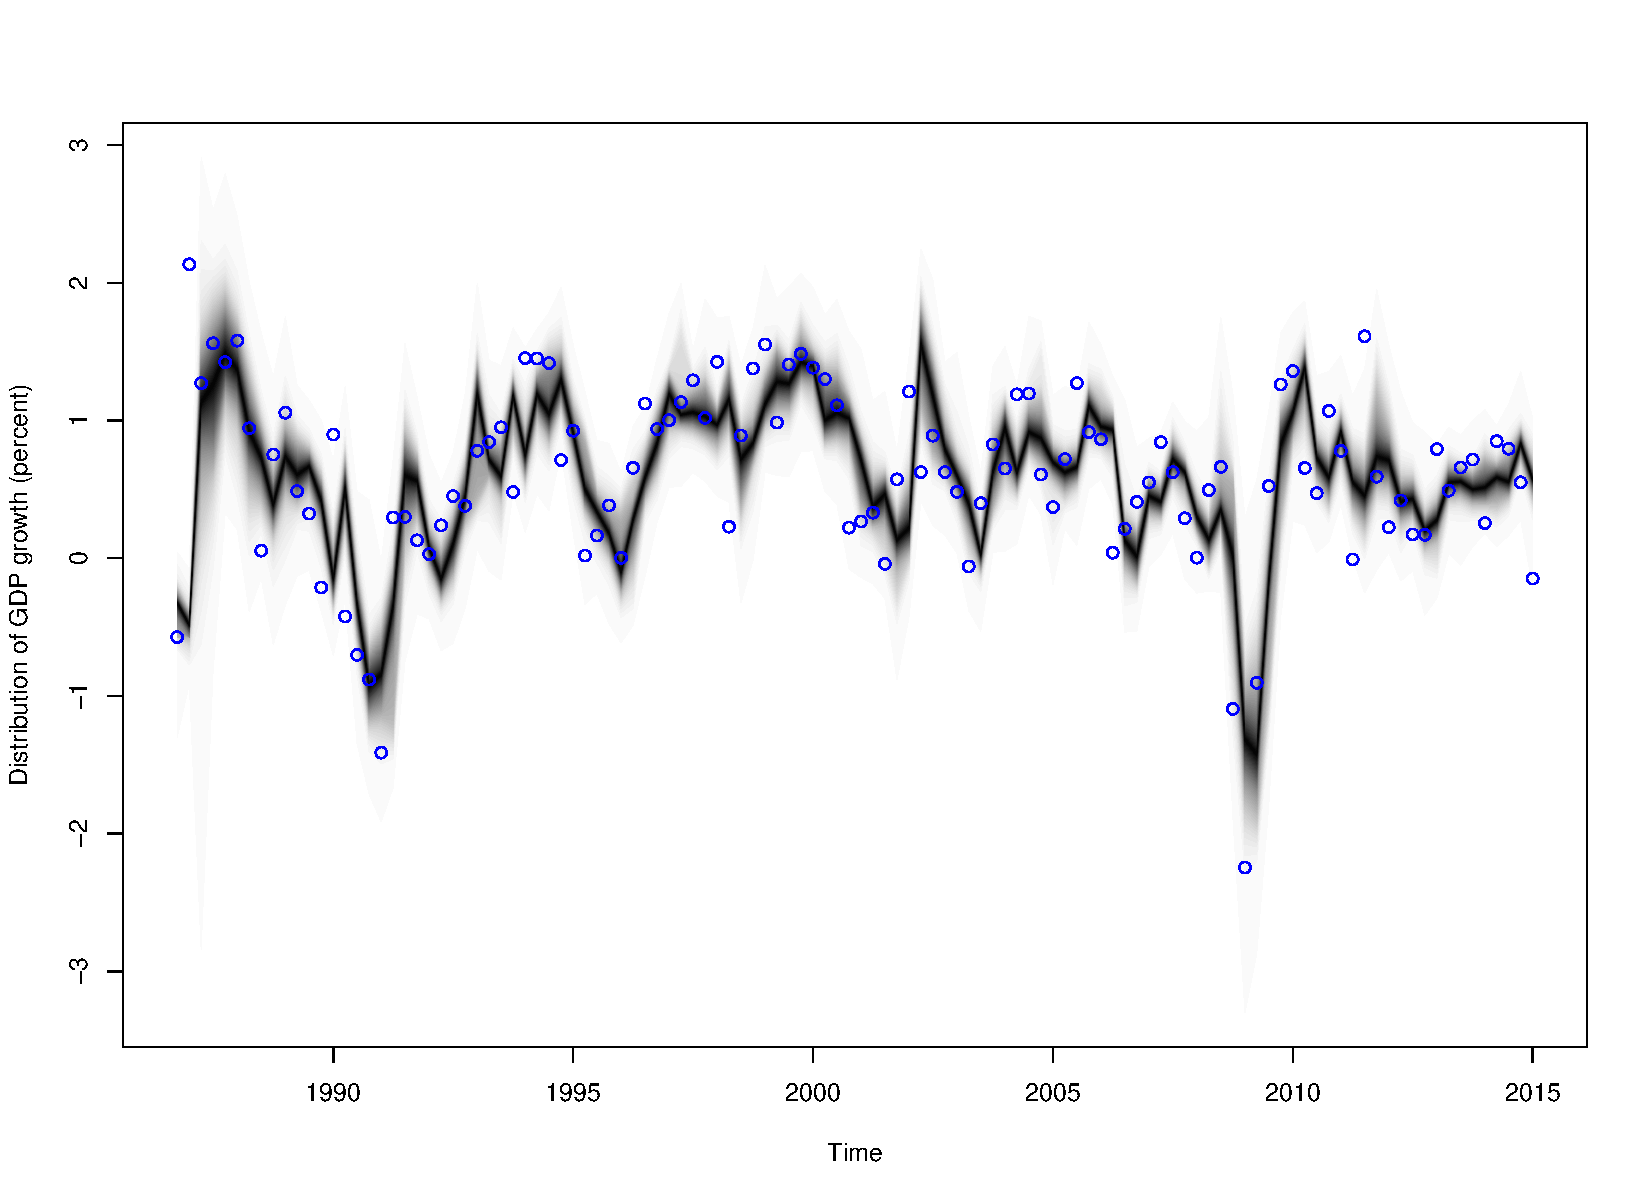
\includegraphics[width=0.6\linewidth]{Figures/forecast_distribution}
\caption{Distribution of one step ahead forecast for observation}
\label{fig:forecast_distribution}
\end{figure}



Figure  ~\ref{fig:forecast_distribution} shows the distribution of one step ahead forecast for observation. The distribution of one step ahead forecast for period $t$ is  made by using the value of GDP growth at $t-1$ and the observed covariates in regression component at time $t$. In Figure~\ref{fig:forecast_distribution}, the blue circle dots are observed GDP growth rate. The median of the distribution of forecast is colored black. To show the distribution, each 1\% quantile away from the median is shaded slightly lighter, until the 99th and 1st percentiles are shaded white. Figure  ~\ref{fig:forecast_distribution} shows the distribution of forecast is close to the observation except in some peculiar period such as 2007 -2008 financial crisis period.


 

When we get the observation of GDP growth rate at time $t$, we can update the \textit{posterior} states at time t; 
$$ \alpha_t|GDP^t \sim N(m_t, C_t) $$ 
where $m_t =  a_t + R_t  f_t^\prime Q_t^{-1} (y_t - f_t)$, $y_t - f_t$ is the forecast error, and $C_t = R_t - R_t F_t^\prime Q_t^{-1} F_t R_t$ \cite{Petris2008}.


Figure  ~\ref{fig:states_distribution} shows that the posterior distribution of state of target variable GDP growth rate has much less variance than one step ahead forecast after the correction of forecast error. The weight of the correction term is given by the gain matrix $K_t = R_t  f_t^\prime Q_t^{-1}$. A close look at Figure  ~\ref{fig:states_distribution} shows us that after the correction, the posterior distribution of state is much closer to the observation than the one step ahead forecast. 




\begin{figure}[h]
\centering
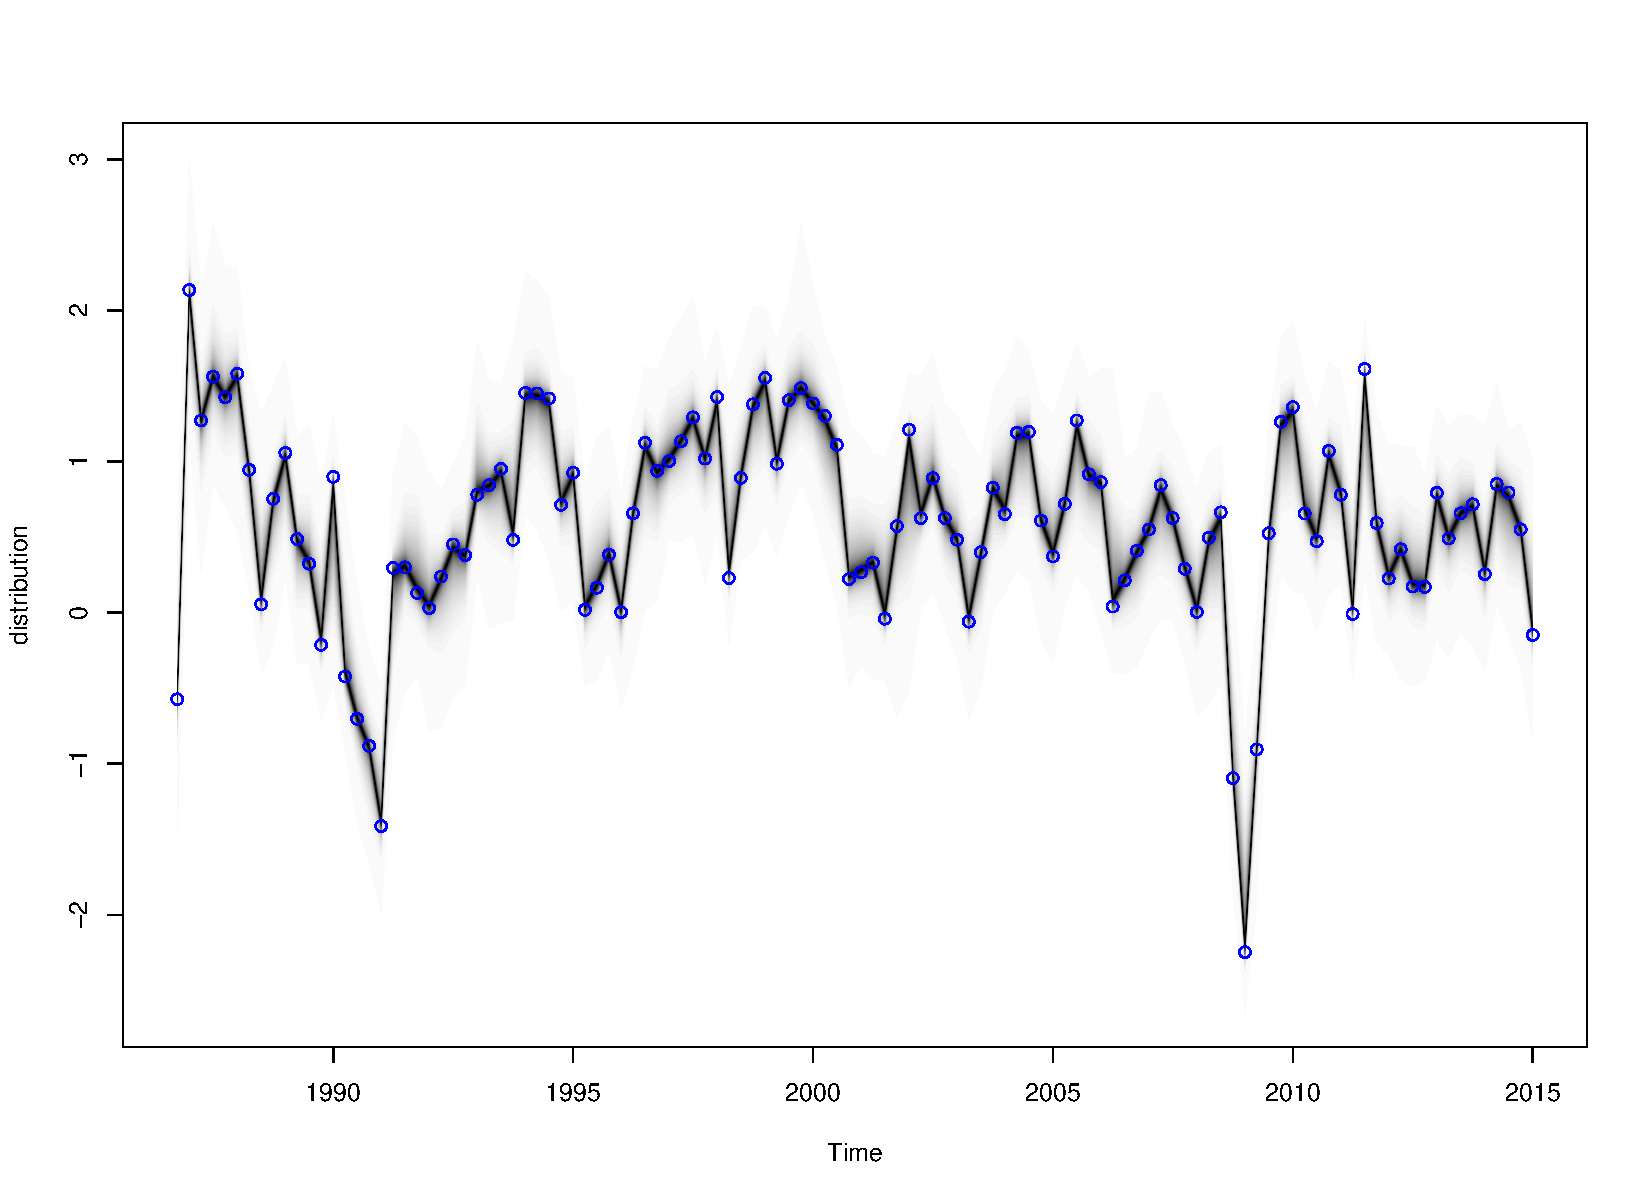
\includegraphics[width=0.6\linewidth]{Figures/states_distribution}
\caption{Posterior distribution of states}
\label{fig:states_distribution}
\end{figure}




\subsection{Diagnostic of the model}

The difference also shows between residual and forecast error. The residual is the difference between posterior state and observation, and the forecast error is the difference between one step ahead forecast and observation. 


\begin{figure}[h]
	\centering
	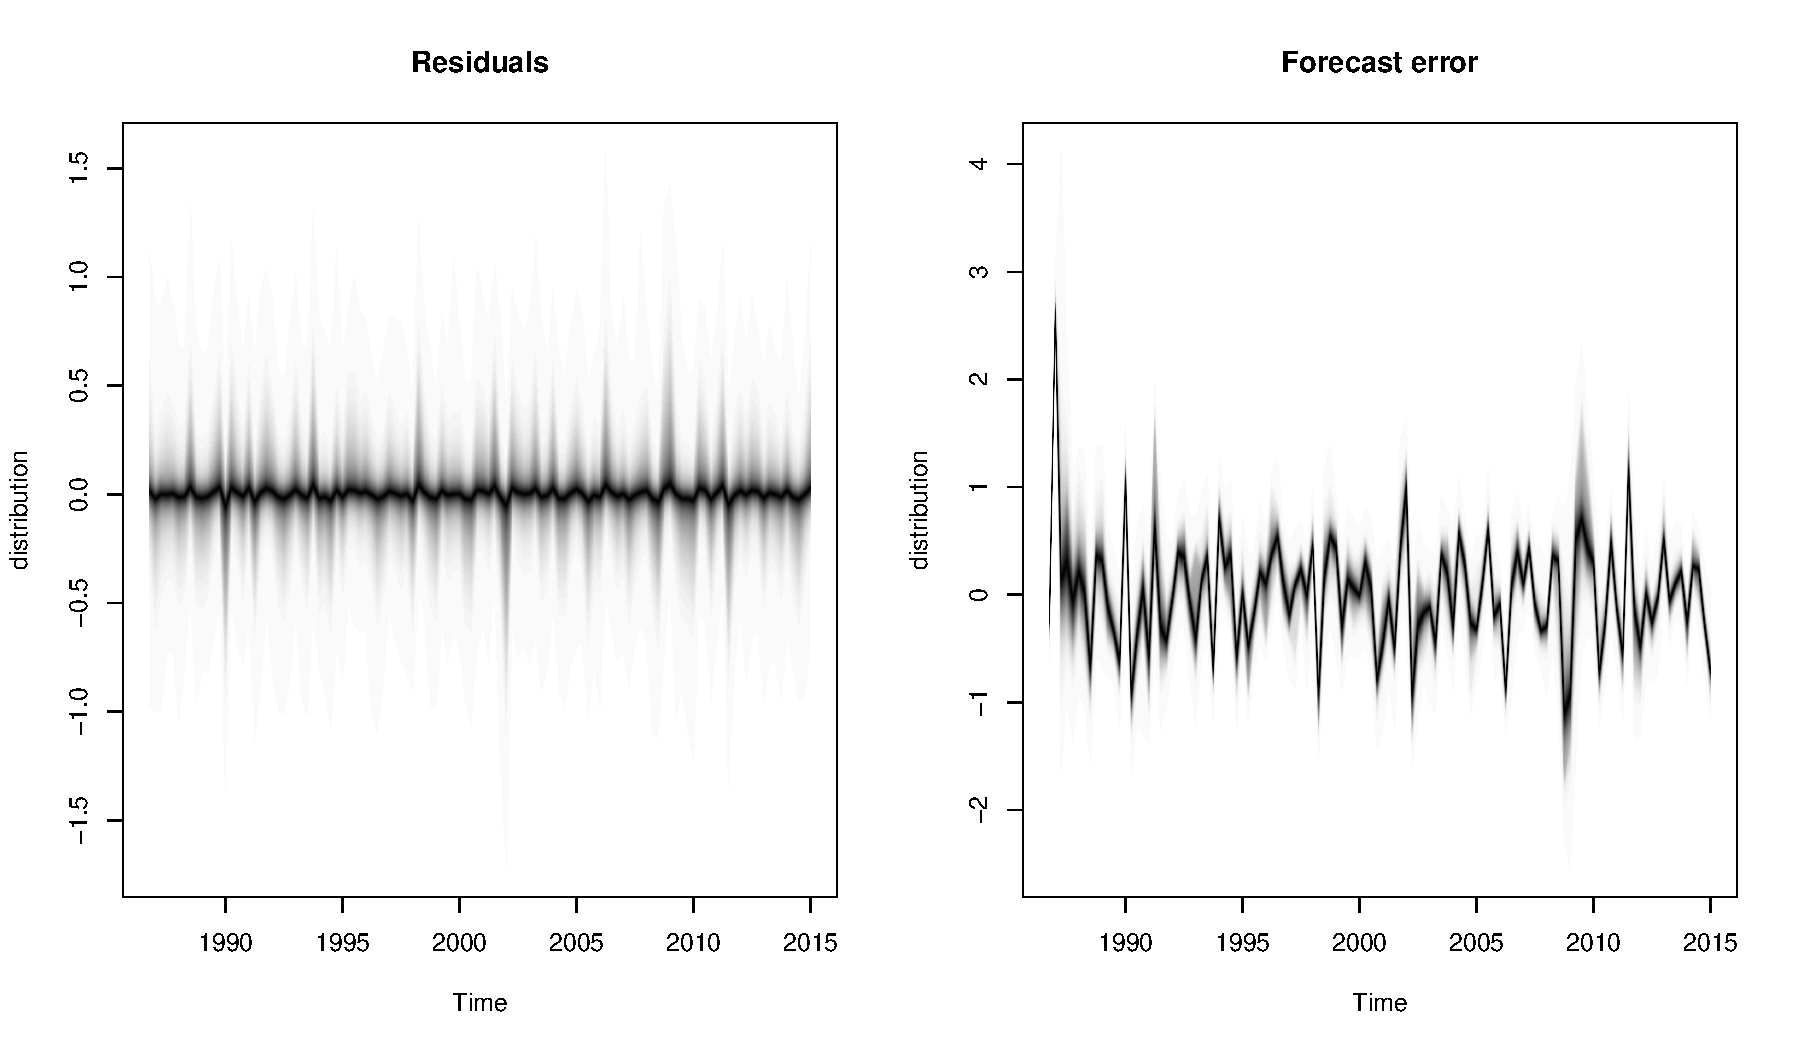
\includegraphics[width=0.8\linewidth]{Figures/residuals_prediction_errors}
	\caption{The distribution of the residual and forecast error}
	\label{fig:residuals_prediction_errors}
\end{figure}

Figure  ~\ref{fig:residuals_prediction_errors} shows the variation of forecast errors are wider than the variation of residuals. Both are center at zero.  

\begin{figure}
	\centering
	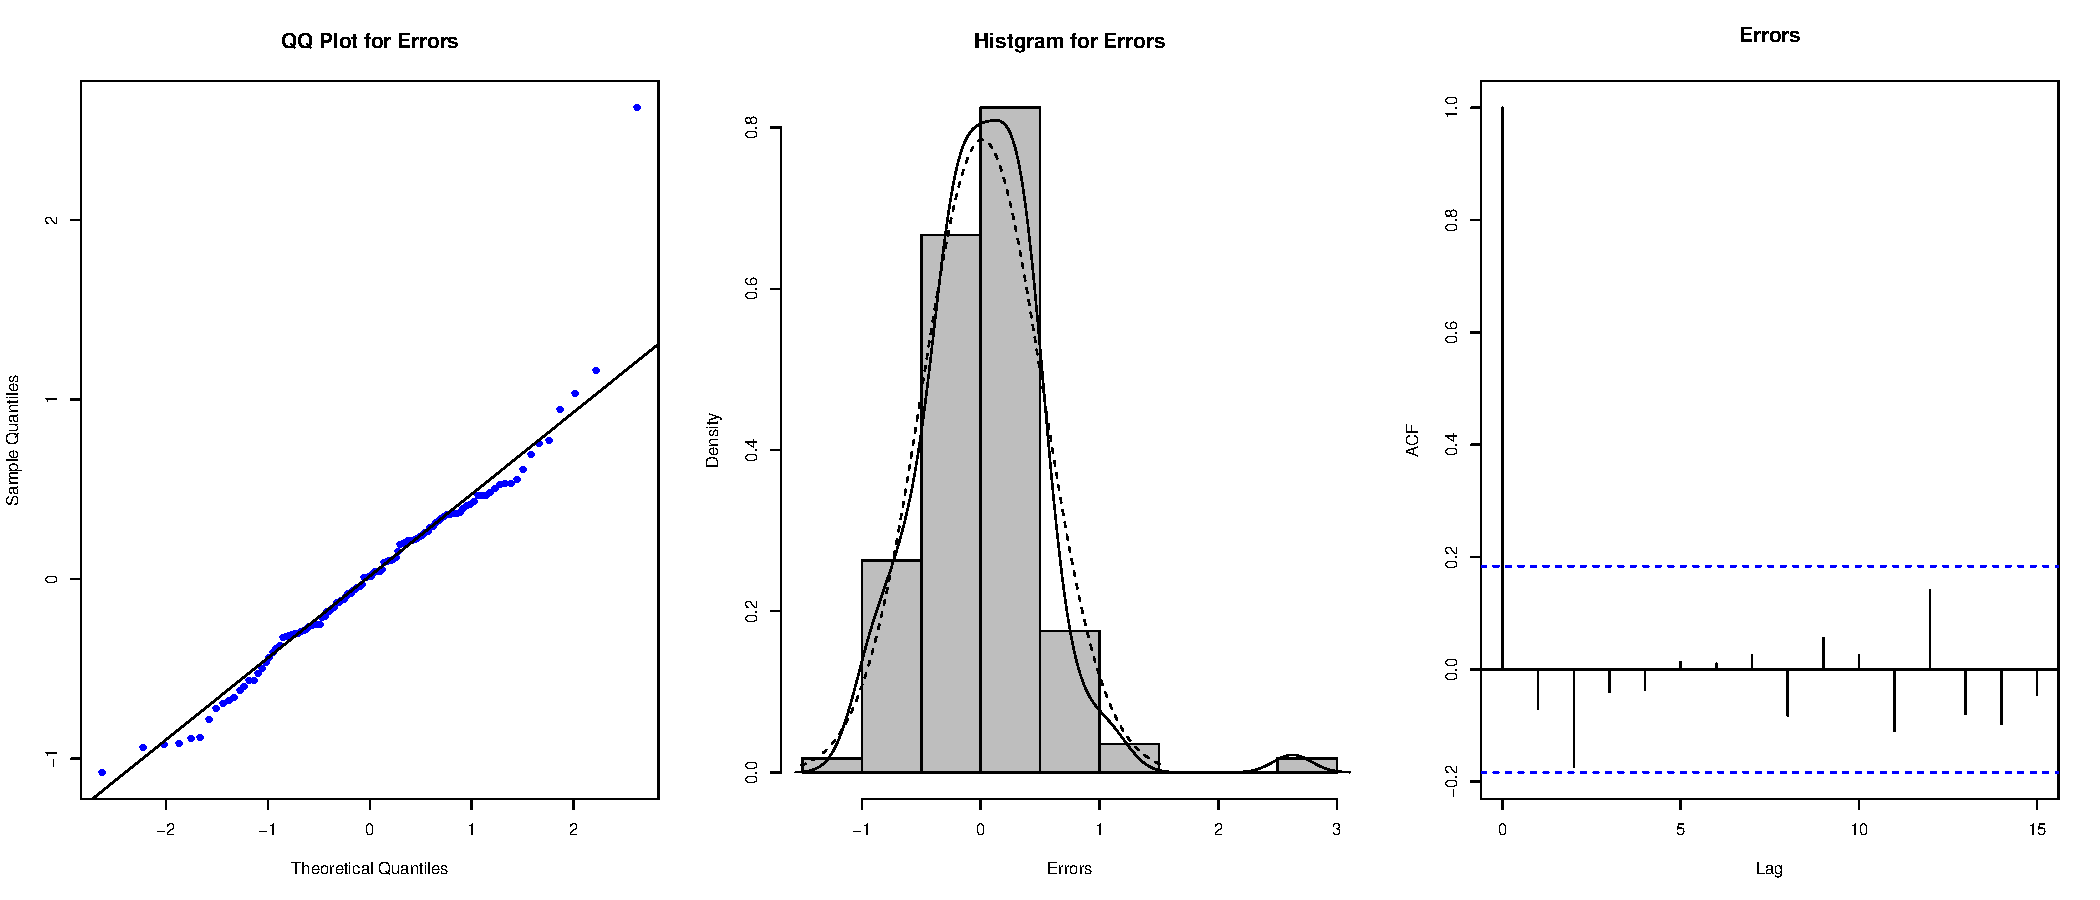
\includegraphics[width=1\linewidth]{Figures/errors3_hist}
	\caption{QQ plot, histogram, and ACF for one step ahead forecast errors}
	\label{fig:errors_hist}
\end{figure}


Figure  ~\ref{fig:errors_hist} shows the distribution of one step ahead forecast errors is very close to normal distribution; however, it does not pass Shapiro-Wilk normality test. The residual does  pass the Box-Ljung test, and the residuals are not autocorrelated, which also can be verified by the ACF diagram in Figure  ~\ref{fig:errors_hist}.    


\begin{figure}
	\centering
	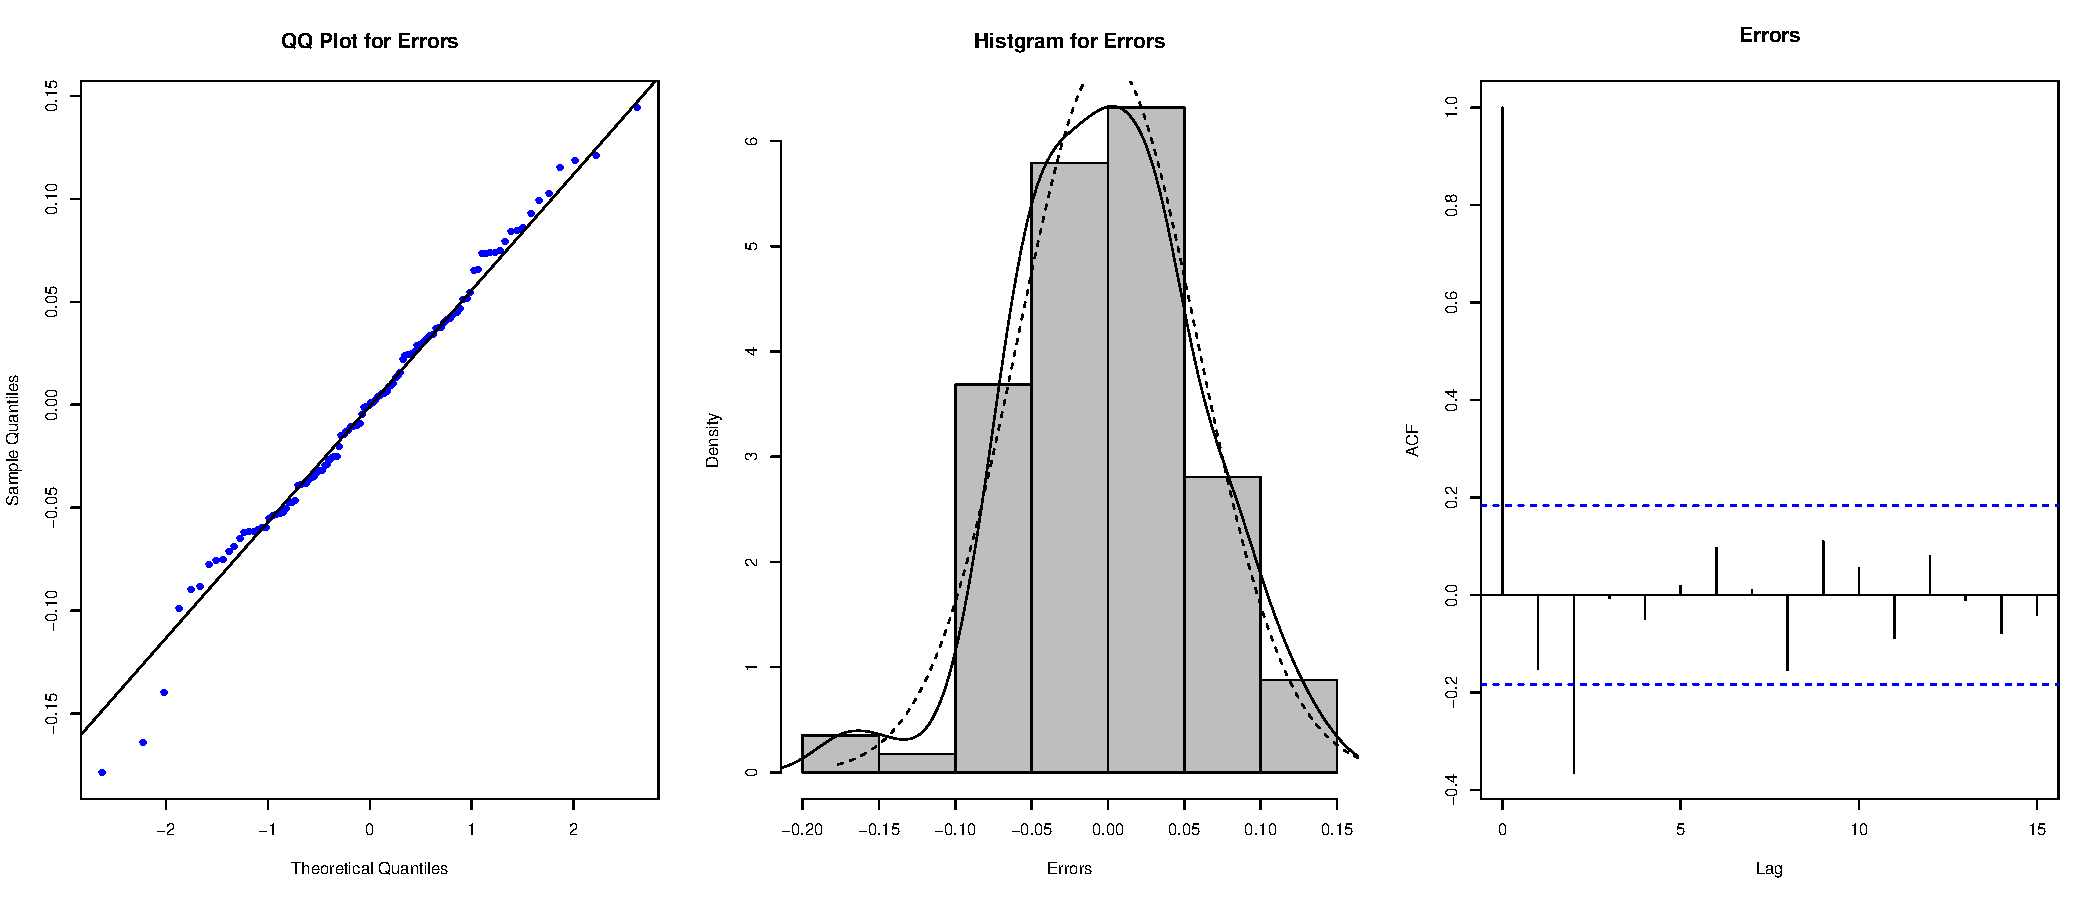
\includegraphics[width=1\linewidth]{Figures/residuals_hist}
	\caption{QQ plot, histogram, and ACF for residuals}
	\label{fig:residuals_hist}
\end{figure}


Figure  ~\ref{fig:residuals_hist} shows the distribution of residuals is almost normal ,which verified by the Figure  ~\ref{fig:residuals_hist}. And it does pass Shapiro-Wilk normality test. The residuals does not pass the Box-Ljung test, and the residuals are autocorrelated, which also can be verified by the ACF diagram in Figure  ~\ref{fig:residuals_hist}.    


\subsection{Contributions of components for GDP growth}

In our model, trend, AR terms and regression are three components besides the irregular error term. 
Figure  ~\ref{fig:components} shows how much variation in GDP growth can be explained by trend and regression component. In Figure  ~\ref{fig:components}, the AR term is relative stable, and the trend component is more volatile. The regression component demonstrates more variation than the trend, which can help to capture the structural break or turning points in the  dynamics of the GDP growth. 


\begin{figure}[h]
	\centering
	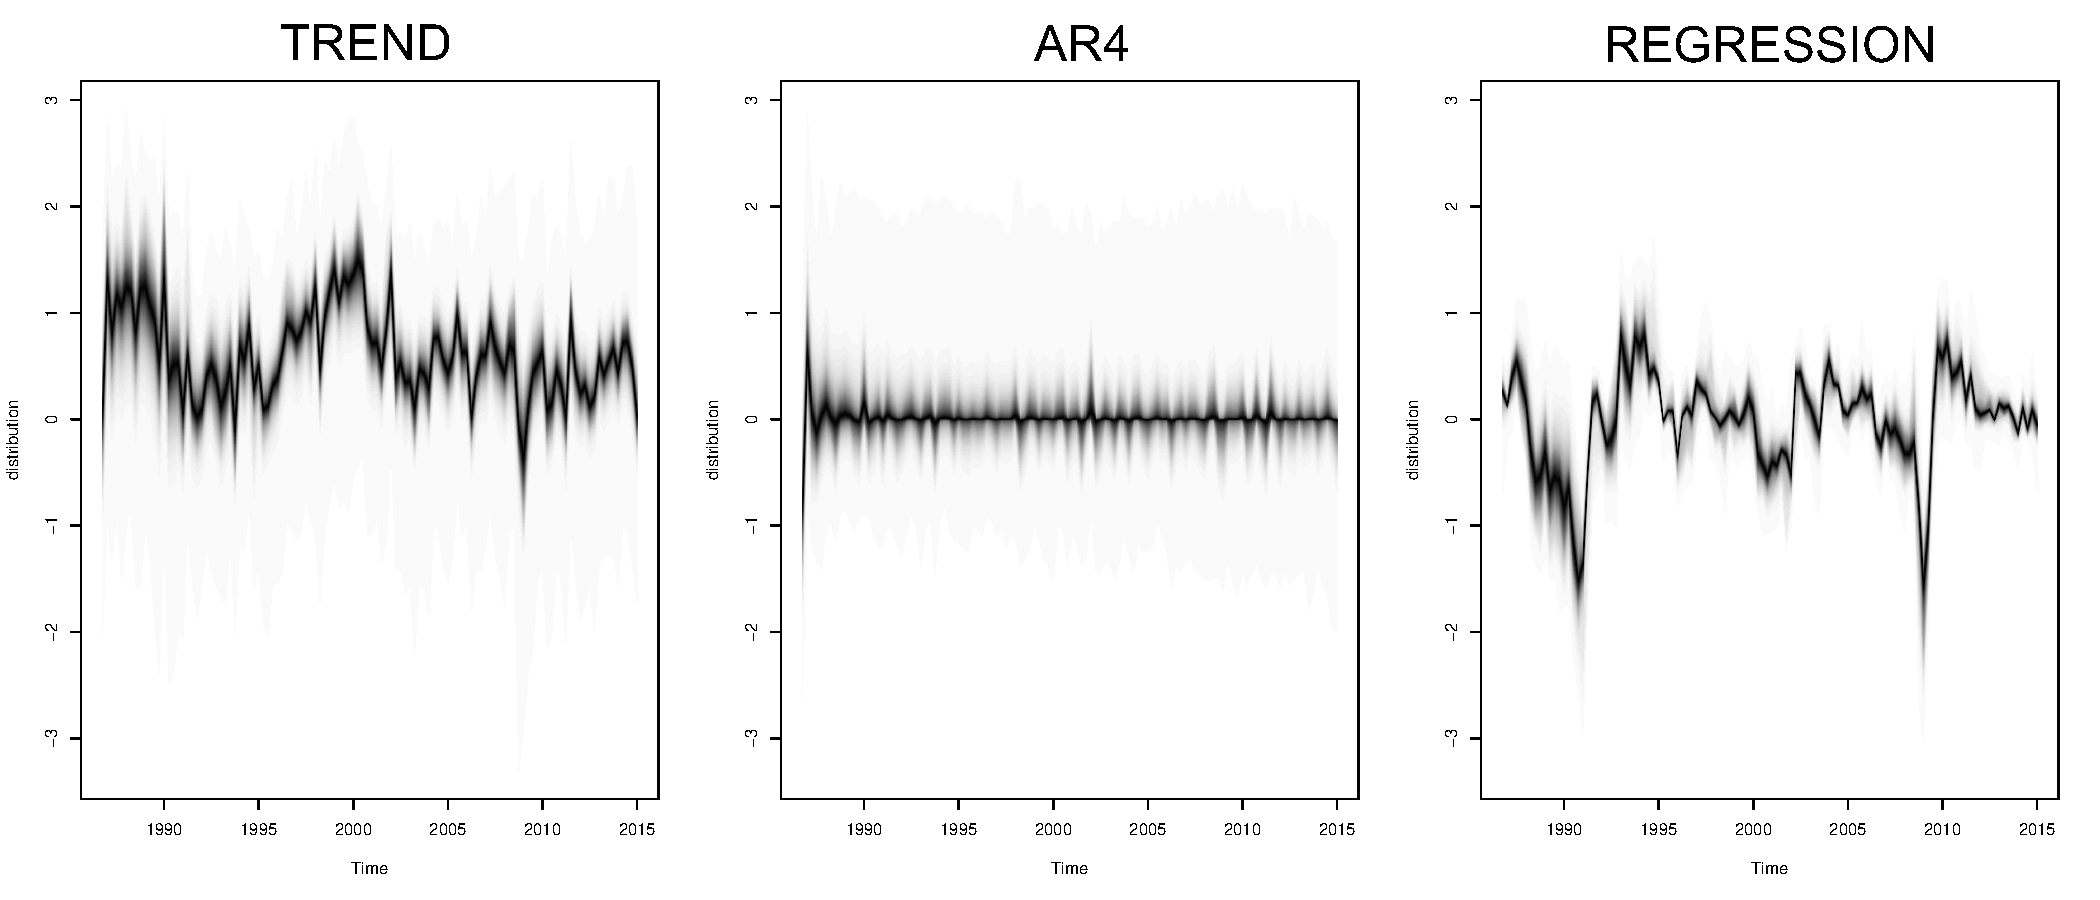
\includegraphics[width=1\linewidth]{Figures/components}
	\caption{Contributions to state for GDP growth}
	\label{fig:components}
\end{figure}




\subsection{The cumulative one step ahead forecast error for two models}

In order to illustrate the value of leading macroeconomic predictors, we fit a generalized local trend and AR(4) model without regression component and compare it with our model3.  The cumulative sum of the absolute values of the one step ahead forecast errors for the two models shows in Figure ~\ref{fig:cumulative_errors}. The model3 performs better, especially during the financial crisis of 2008–2009, which emphasizes one of the advantage of BSTS-U-MIDAS: robust to change points and structural break.  


\begin{figure}
	\centering
	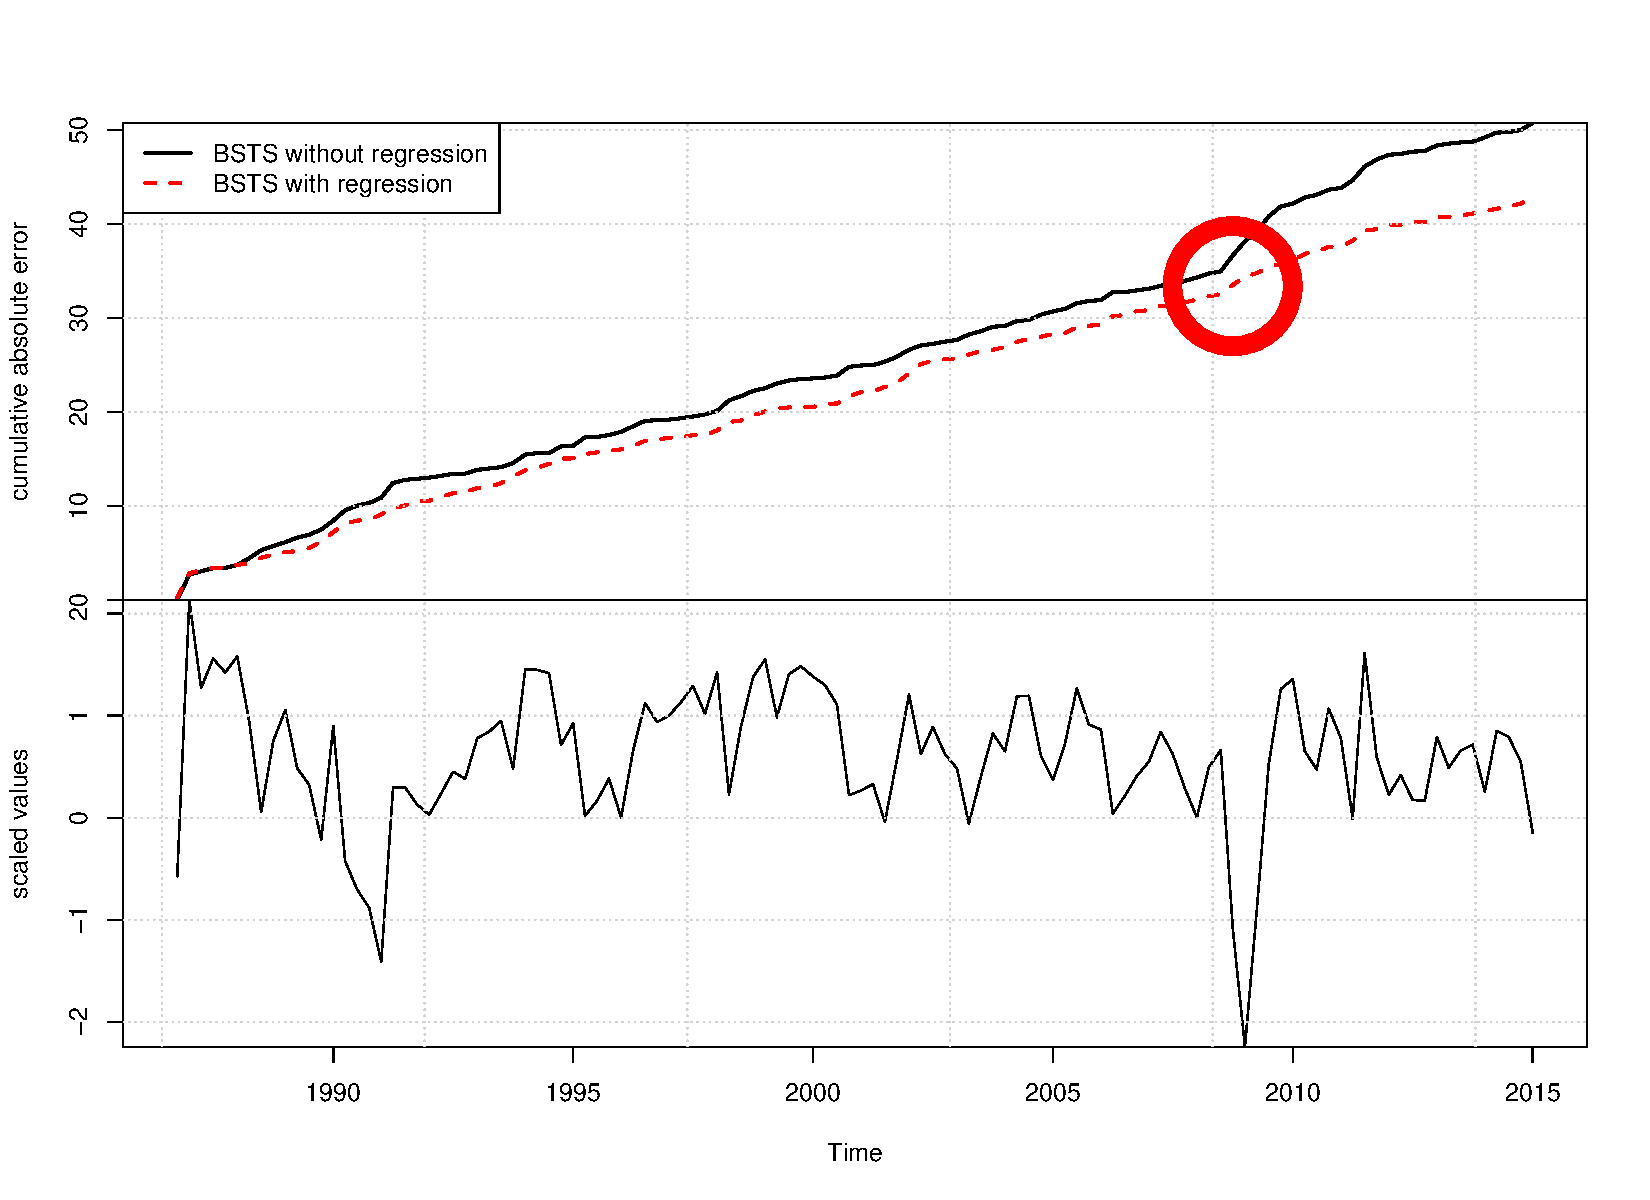
\includegraphics[width=0.6\linewidth]{Figures/cumulative_errors}
	\caption{The cumulative one step ahead forecast error}
	\label{fig:cumulative_errors}
\end{figure}


The cumulative sum of the forecast errors for model without regression component jumps when the recession starts. However, the cumulative sum of the forecast errors for model 3 increases in a constant rate. 

The robustness to structural break of the BSTS-U-MIDAS could be very helpful for us to predict recession or booming. 

\subsection{The predictors with large inclusion probability}

Another thing of interest in our forecast  is to find out which predictor is significant according to its ability for helping predict the variation of GDP growth in Canada.


\begin{figure}[h]
	\centering
	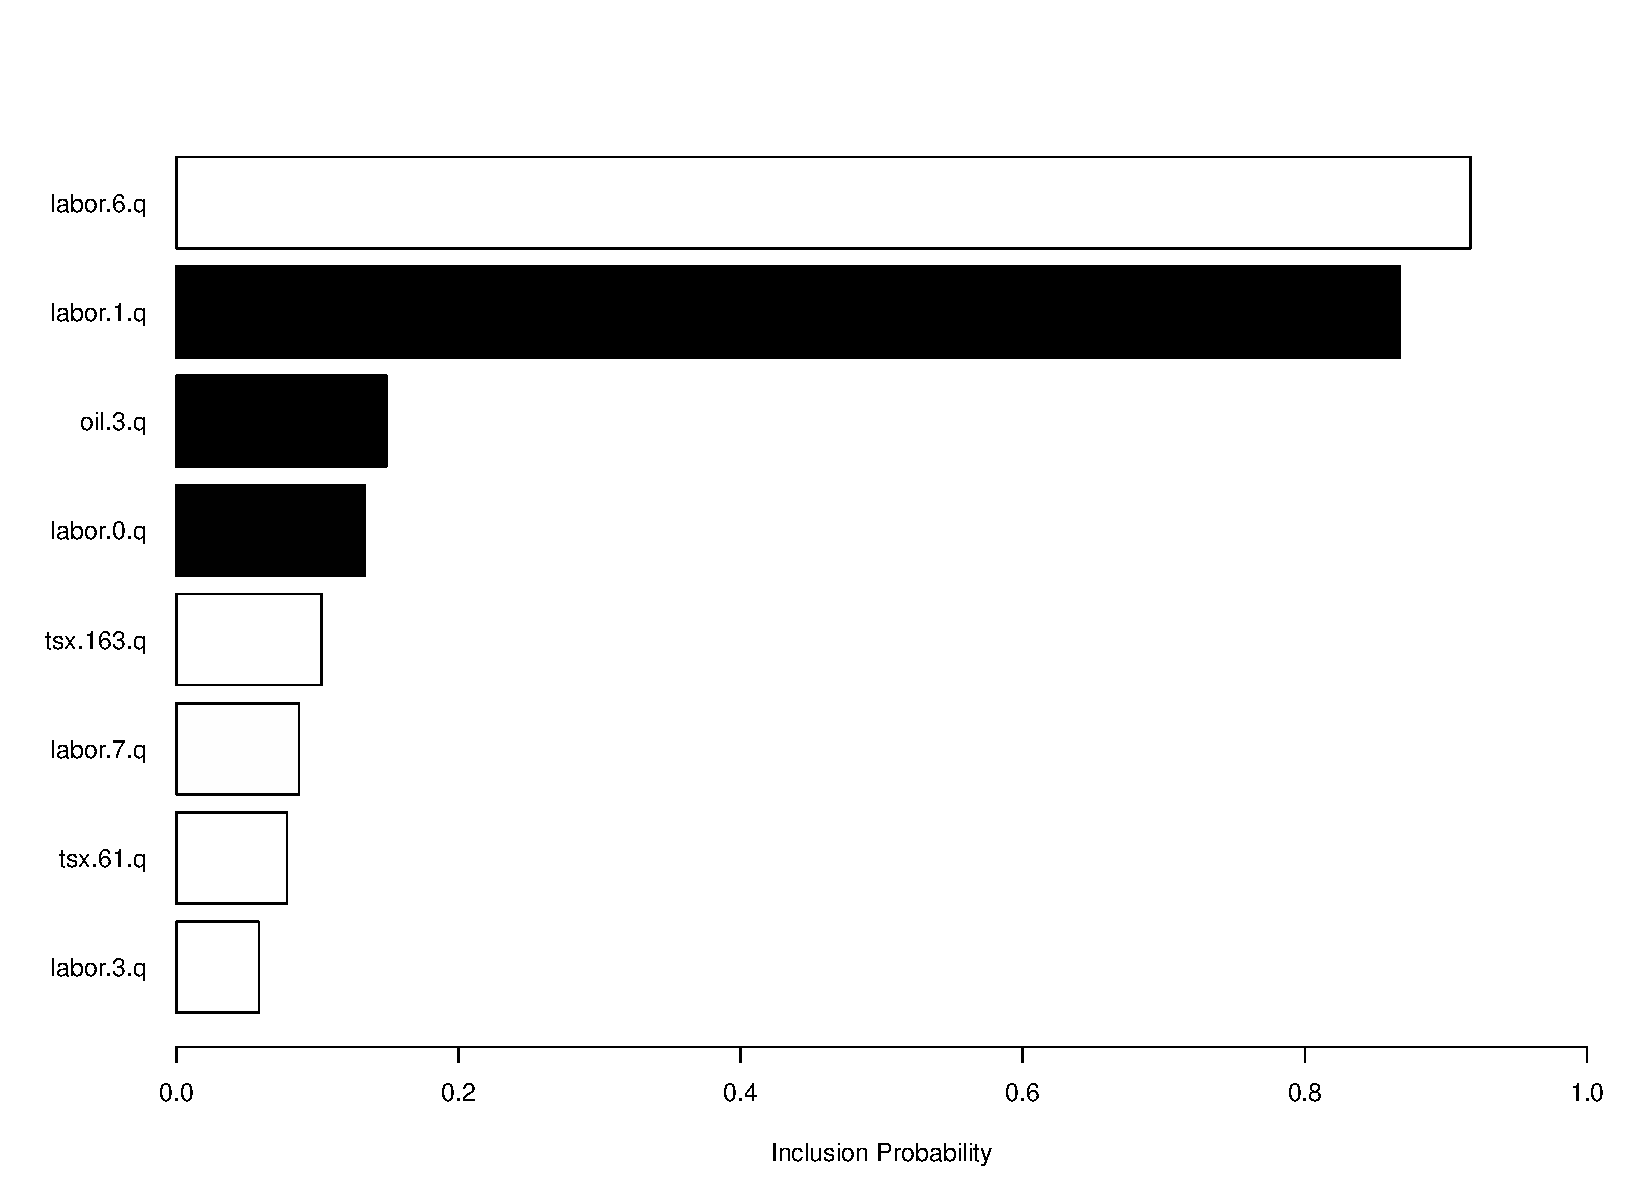
\includegraphics[width=0.7\linewidth]{Figures/Coefficients}
	\caption{Predictors with inclusion probability}
	\label{fig:Coefficients}
\end{figure}


Figure ~\ref{fig:Coefficients} shows the predictors with inclusion probability greater than 5\% . A white bar indicates that the predictor has a positive relationship with target variable, and a black bar indicates a negative relationship. The size of the bar represents inclusion probability. 

The unemployment rate is labeled as "labor", TSX stock market index return is labeled as "tsx", and oil price return is labeled as "oil". The "labor.0.q" represent the most recent observation for unemployment rate. In our model, "labor.0.q" is unemployment rate for the last month in the reference quarter. "labor.6.q" is fourth month before the reference quarter.For example, the last target quarter is first quarter 2015, and then the last "labor.0.q" observation is the  unemployment rate for March 2015. The last "labor.6.q" is the unemployment rate for September 2014. 

Likewise, for daily data, "oil.3.q" is oil price return (log difference of oil price) in May 25, 2015, three days before May 28, 2015. "tsx.61.q" is stock market return sixty one business days before May 28, 2015, one day in March 2015.  The locations of predictors with high probability on time table  are illustrated in Figure ~\ref{fig:MonthQuarterYear}. 


\begin{figure}
	\centering
	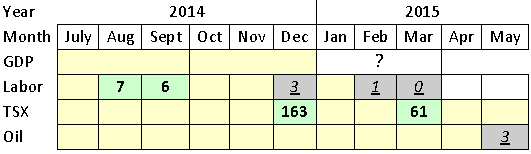
\includegraphics[width=0.7\linewidth]{Figures/MonthQuarterYear}
	\caption{Predictors with high probability on time table}
	\label{fig:MonthQuarterYear}
\end{figure}



The signs of the coefficients of other predictors mostly meet our anticipation. The spread of long term and short term bonds interest and unemployment rate is negatively related to GDP growth. The effects of return of TSX index and oil price are much more complicated. 

In our model, we do not choose variables and their lags according to AIC or BIC. Instead, the model uses SSVS algorithm to choose which variable should be included in the regression. In the process of iteration, the model calculates the proportions of estimated models including the predictors as the marginal inclusion probabilities.












\begin{figure}[p]
	\centering
	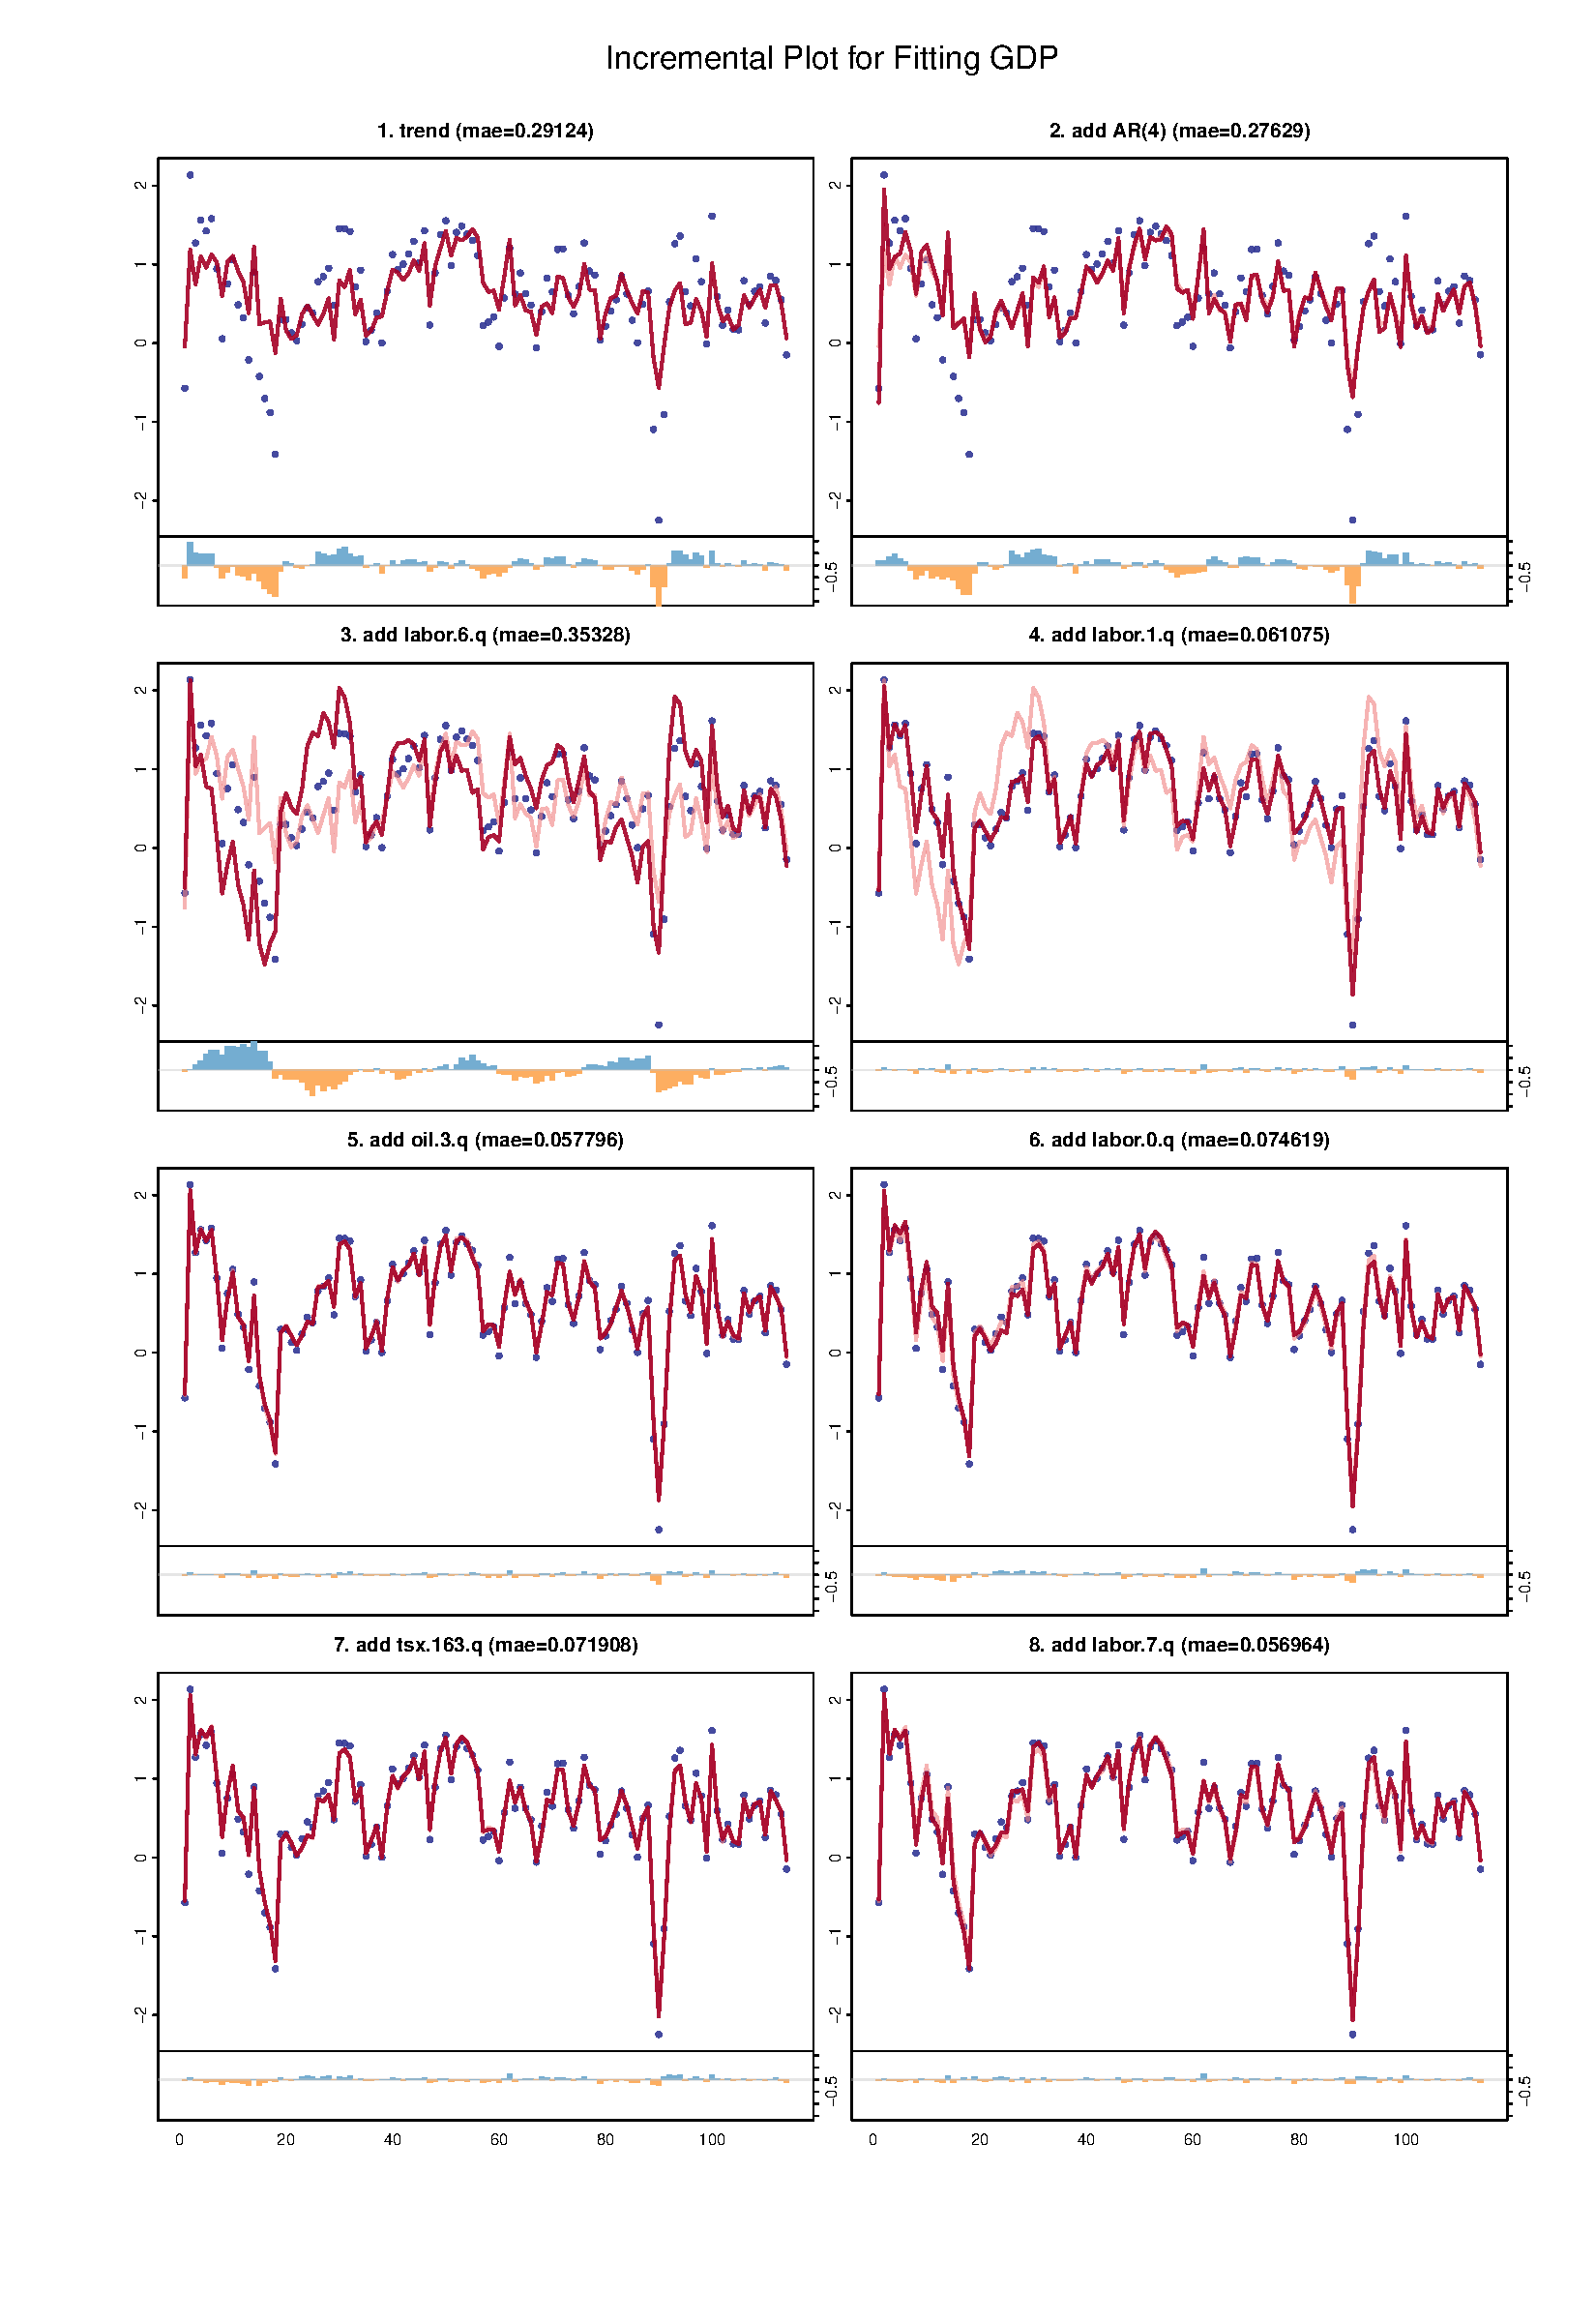
\includegraphics[width=1\linewidth]{Figures/GDPincremental}
	\caption{Decomposition of forecast for GDP growth}
	\label{fig:GDPincremental}
\end{figure}

(This part may not be included in the paper)
Figure ~\ref{fig:GDPincremental} shows the contribution of each state components and predictors to the fit of model. Variables
are ordered by probability of inclusion, mean absolute error is given in title,the faint line in each panel is the previous fit, and residuals are shown at bottom of each panel. 

shows that when we add more predictor in regression the one step ahead forecast better fits the target varialbes except current unemployment (lable as "labor") and the tenth lag of spread (lable as "spread .10").

It is interesting that including "labor" and "spread.10" actually decreases the fit and increases the error. This is coincident to the phenomenon that both of them have negative relationship with target variable. How ever, the combination of these two predictors and other predictors enhance the forecast. 

This phenomenon shows that individually including one specific predictor may not improve forecasting, but jointly including a set of predictors might improve forecasting a lot. 





The top 4 predictors have over 60\% percent probability to be included in the model. Other predictors are much less likely to be included in the model. It gives us a relative sparse model, which also be verified by the distribution of the size of model in Figure ~\ref{fig:size} 

\begin{figure}[h]
	\centering
	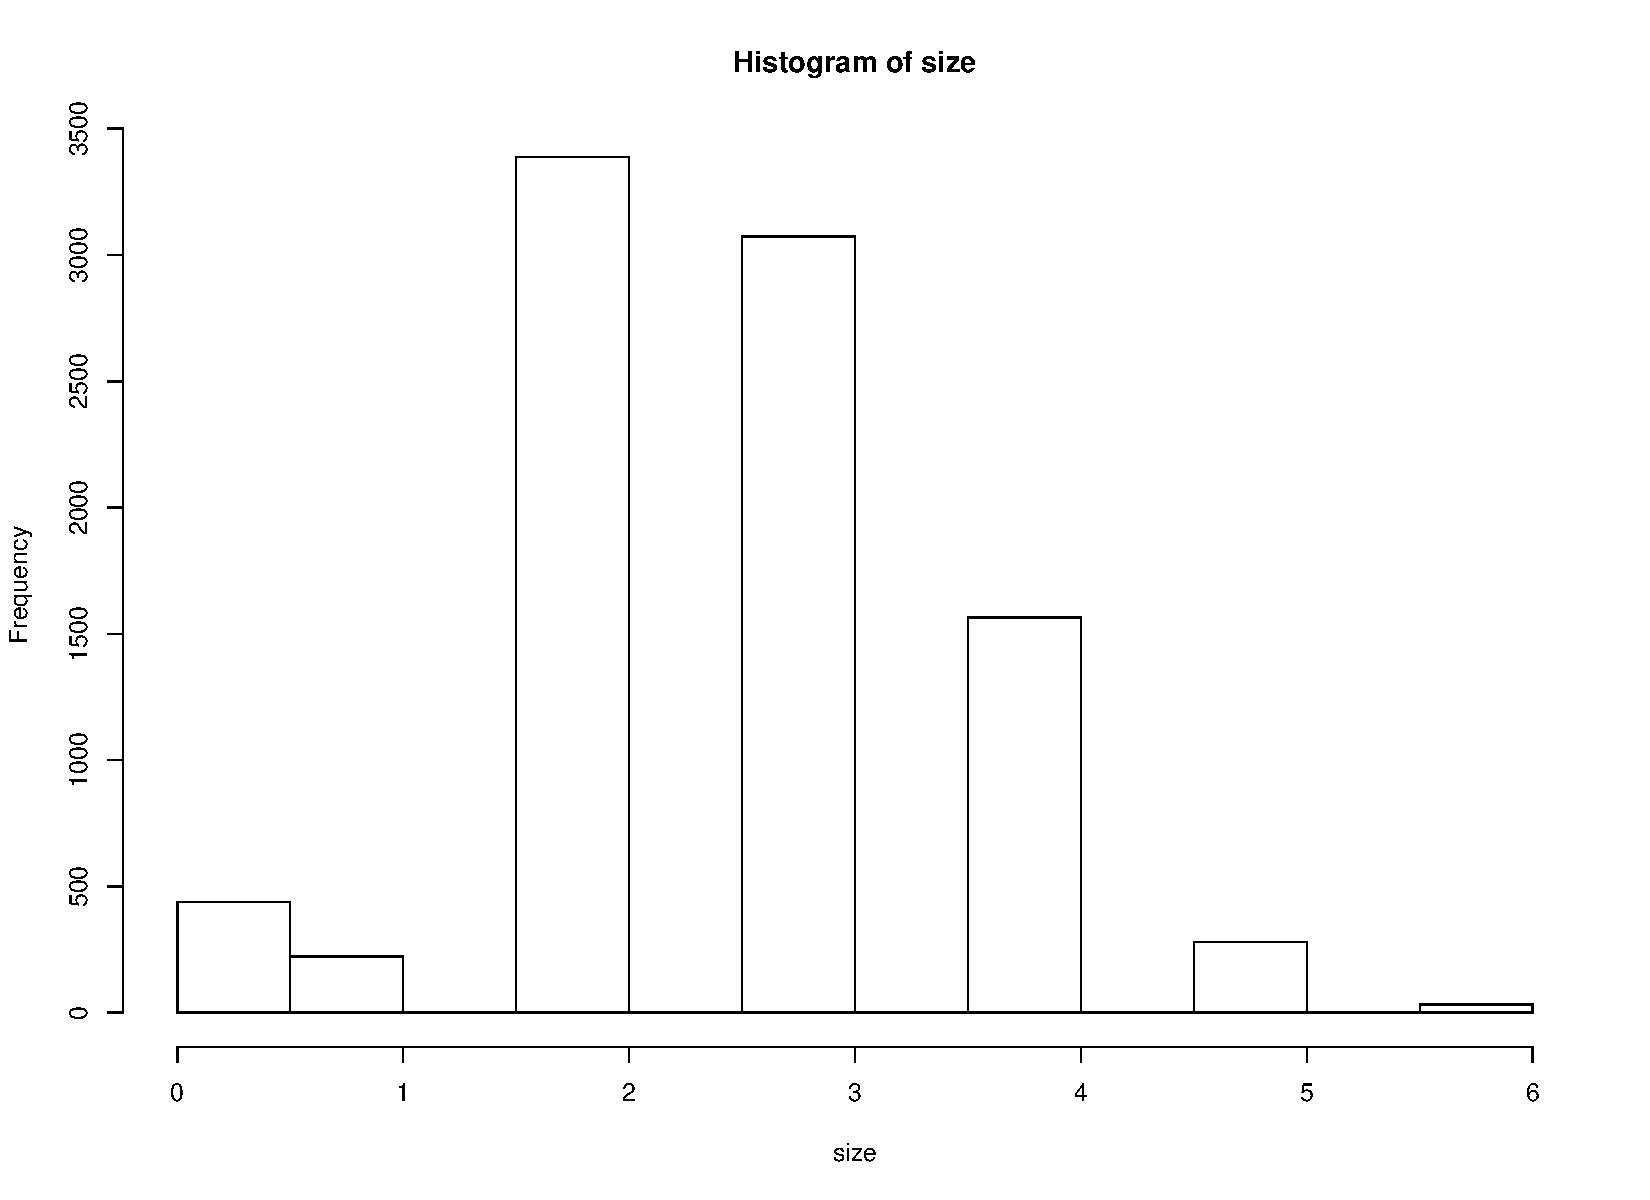
\includegraphics[width=0.5\linewidth]{Figures/size}
	\caption{The posterior distribution of  model size}
	\label{fig:size}
\end{figure}

Figure ~\ref{fig:size} shows the posterior distribution of the number of predictors in the model. We have 288 variables to choose from, and the mean and median number of predictors is 4, and the largest model in the MCMC sample has 6 predictors. The model indeed gives us sparsity.  




It is worth to notice that in second model the residual and forecast error do not change, but in third model, the residual get very small and forecast error get bigger. The explanation could be the extra predictor housing start data in second model does not have much information for improving the performance, however the extra predictor oil price in third model cause the overfit of the model. It also can be verified by the R squared in those models. The R squared in first and second model are about 68\%, and it is 99\% in third model. R squared is calculated by formula $ R^2 = 1- var(residual)/var(target)$. The distribution of residual and forecast error is left in Appendix C.



\subsection{The contribution of the predictors with large inclusion probability}

Figure ~\ref{fig:BSTSpredictors} shows the co-movement of target variable GDP growth and predictors (see online version for colours). The blue line is the observed GDP growth. Other shaded lines are predictors, and the shading of the lines is weighted by the marginal inclusion probability.

\begin{figure}[h]
	\centering
	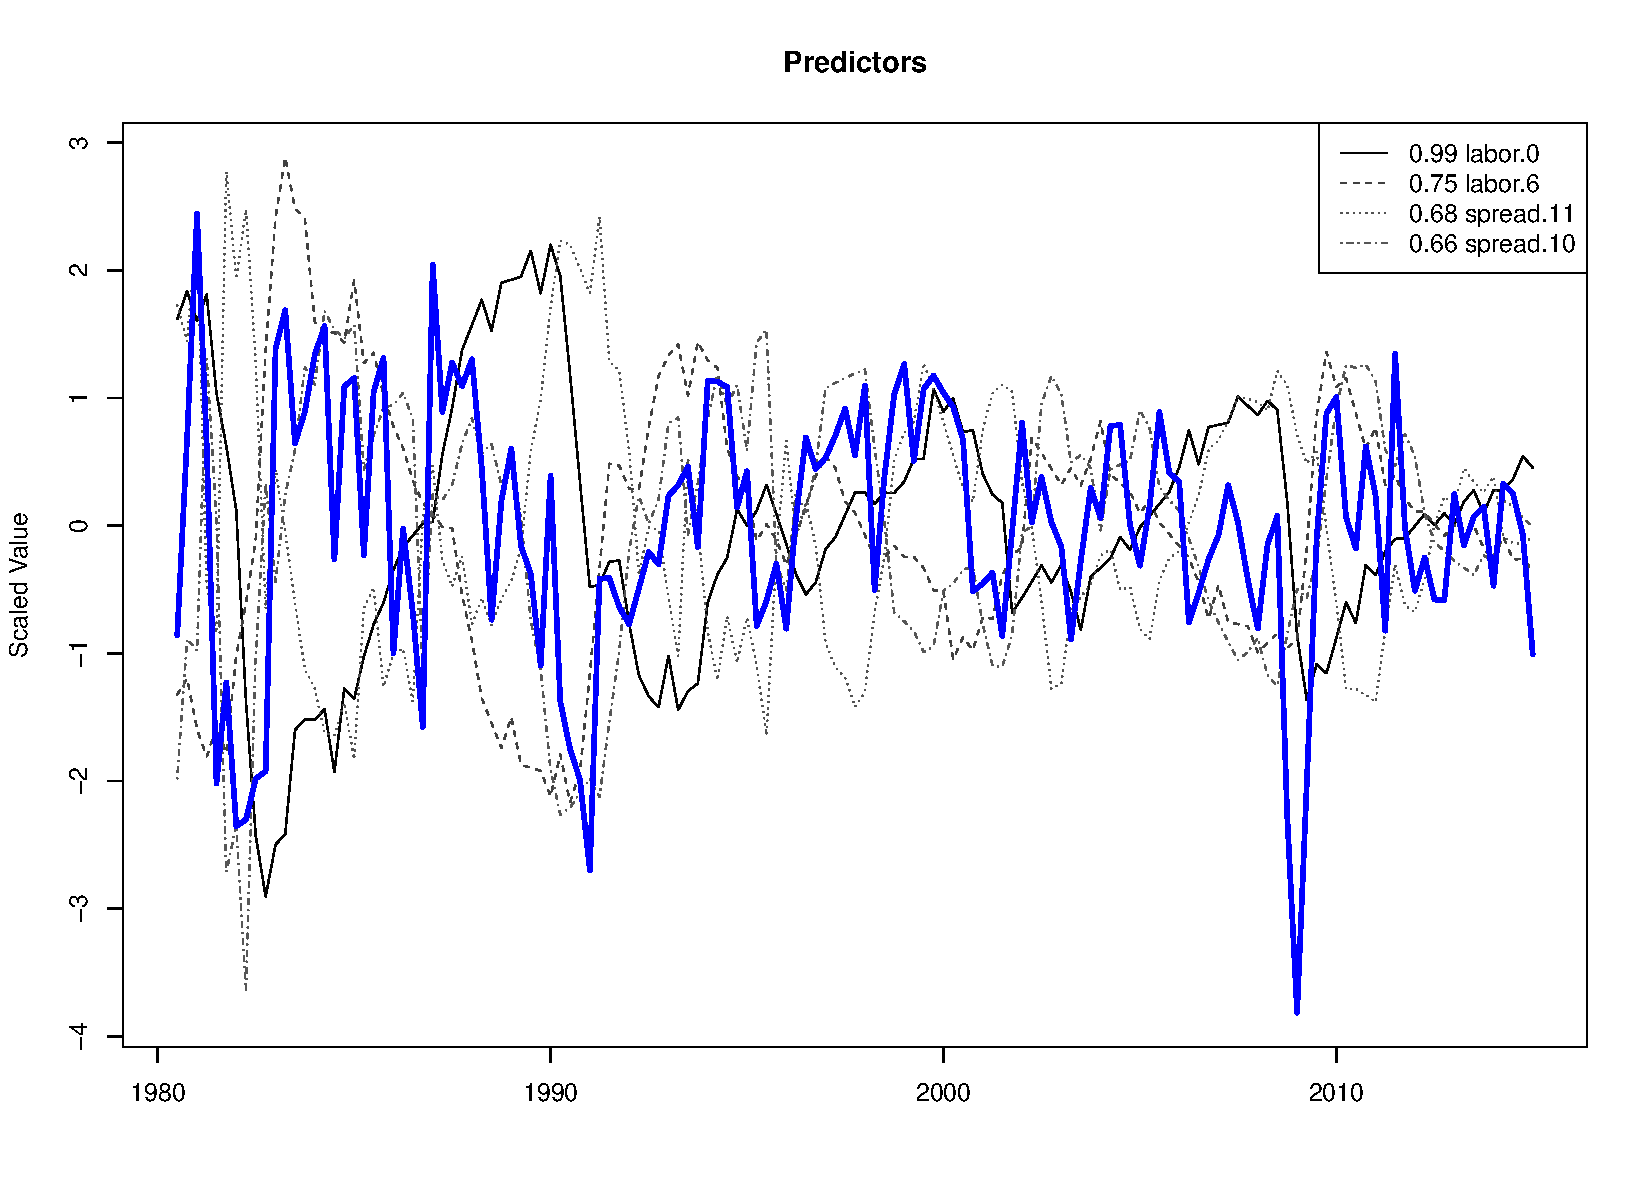
\includegraphics[width=0.9\linewidth]{Figures/BSTSpredictors}
	\caption{Co-movement of target and predictors}
	\label{fig:BSTSpredictors}
\end{figure}

The unemployment rate "labor.0" in the last month of the target quarter has negative relation with GDP growth in the target quarter. And its change is a little ahead the change in GDP growth. When the unemployment gets its peak, the GDP growth is going to touch its lowest point. The same phenomenon occurs in spread between long government bond and short bond rate 9 month before the target quarter "spread.11". The signs of "labor.0" and "spread.11" meets our anticipation according to economics theory. The higer unemployment rate and spread between long bonds and short bonds interest rate are, the lower GPD growth is.  
However, 

\subsection{The combination of predictors with large inclusion probability}









In the graph, "labor.6" means a sixth lag, and "spread.10" means a tenth lag. The numbers of lags are all calculated according to the transformed data $\tilde{x_i}$. In our case, we have unemployment rate up to March 2015, so "labor.6" means a skipping sampled monthly unemployment rate for third month in a quarter, and the first observation for "labor.6" starts at September 2014. "spread.10" follows the same pattern, and since we have spread between ten year and three month government bonds interest rate up to February, the starting point for it is April, 2014. The TSX stock market return labeled as "tsx". The "tsx.148" represents the one hundred forty eighth lag. We have TSX stock market return data up to May fifth 2015, so "tsx.148" is a quarterly skipping sampled variable and starts at about October twentieth 2014. 

All these predictors are 6-10 months away from the most recent observations and 2-3 month away from the beginning of the target quarter we forecast for. Those evidences show short term shocks, the leads in current quarter and lags in previous, have stronger impact on target variable.

It is interesting that "labor" and "labor6" both are top predictors, but have opposite impact on GDP growth. The same thing happens between "spread.10" and "spread.9". 




In Figure ~\ref{fig:Coefficients}, the house starting does not show in the top 10 predictor. The reason might be the data we collect is not representative for housing market. Or the Canadian housing market is relative stable during 1986 - 2015 even though in some short period housing market might have a big impact on Canadian economy. 


 









\section{Comparison between AR(1) and BSTS}



Especially, during the 2008 financial crisis period, the forecast error of BSTS without regression increases rapidly.  The reason might be  there is a big structural break in the target time series during financial crisis period. The dynamic components such as trend change a lot, and the univariate BSTS cannot predict this dramatic change. However, in BSTS without regression model, the signal among those leading predictors help to predict the economic force which drive the dramatic change in the target variable. \citeA{Petris2008} also mention the same mechanism in which a regression model is more appealing than an univariate dynamic linear model. Especial when the model includes leading predictors, the regression model helps to find the change points and structure breaks.

Due to the same reason, the AR(1) model is outperformed by the BSTS model. And the similarity between performance of BSTS without regression model and that of AR(1) model also show that both models equivalent in some sense. AR(1) can be cast in the form of univariate BSTS model. Both models only use the information of target variable and have difficulty time to predict the structure change in target variable.





We take data from 1980/04/01 to 2003/01/01 as training period and 2003/04/01 to 2015/01/01 as test periods. 



\begin{figure}[h]
\centering
\includegraphics[width=0.7\linewidth]{Figures/bsts_arima}
\caption{GDP Growth, BSTS and ARIMA Forecast}
\label{fig:comparison}
\end{figure}




Figure ~\ref{fig:comparison} shows the forecasting performance from BSTS model is better than that from AR(1) model during the financial crisis period(2007-2010). 




In Figure ~\ref{fig:comparison}, ARIMA(1,0,0) is chosen by automatic arima algorithm in Forecast package in R \cite{Hyndman2015}. The forecast is one step ahead recursive forecast and estimate by arima function in Forecast package in R \cite{Hyndman2015}.  




Figure ~\ref{fig:bsts_boost} shows the forecasting performance from BSTS model is better than that from boosting model during the financial crisis period(2007-2010). 

\begin{figure}[h]
\centering
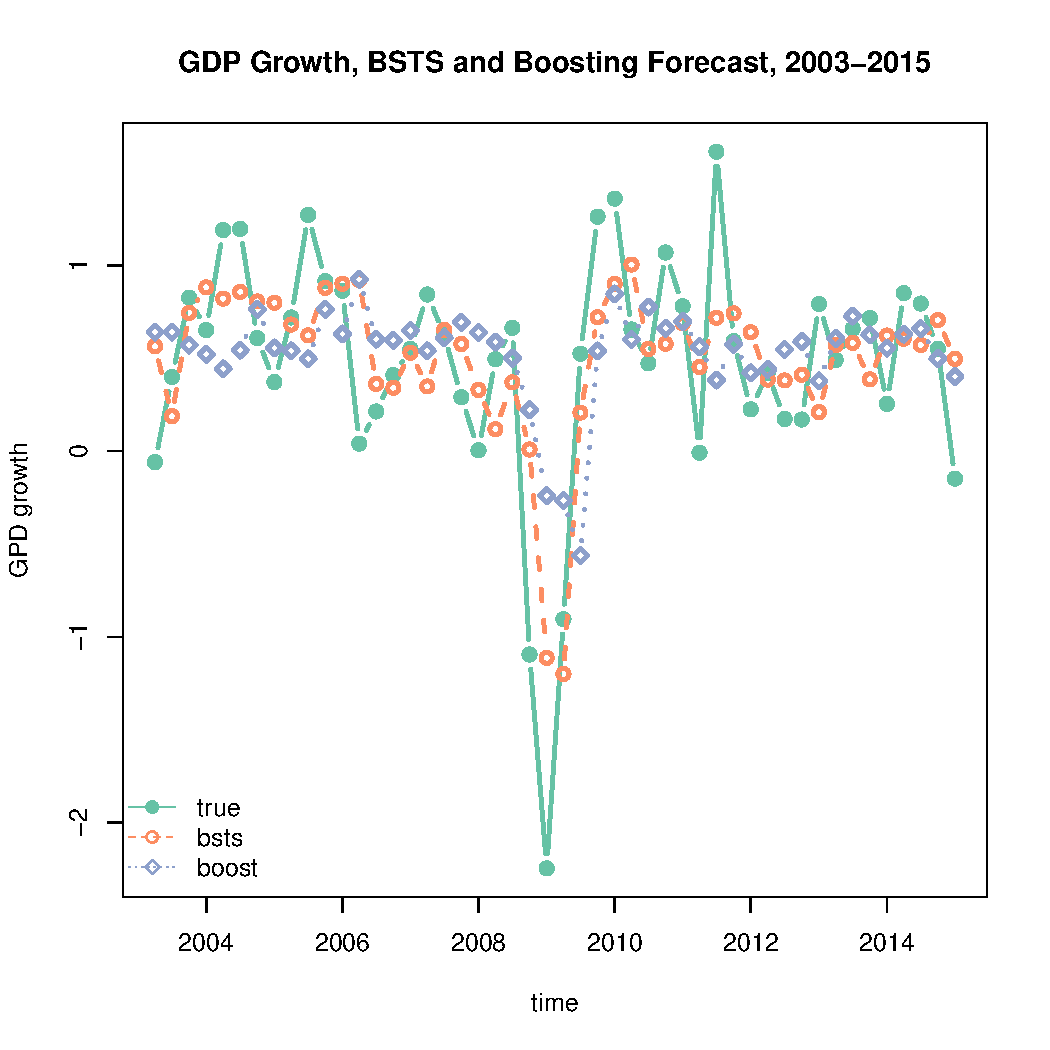
\includegraphics[width=0.7\linewidth]{Figures/bsts_boost}
\caption{GDP Growth, BSTS and Boosting Forecast}
\label{fig:bsts_boost}
\end{figure}



In Figure ~\ref{fig:bsts_boost}, Boosting model is implemented by GBM package in R.  The parameters in GBM model can be found in appendix D.


In order to compare the performance of forecasting, we also calculate the forecasting of level for GDP because the levels of GDP are of interest for our forecast.  

% Please add the following required packages to your document preamble:
% \usepackage{booktabs}
\begin{table}[h]
	\centering
	\begin{tabular}{@{}llllll@{}}
		\toprule
		& ME          & RMSE      & MAE       & MPE       & MAPE     \\ \midrule
		BSTS          & -356.808 &  6804.382 &  5307.138 &  -0.022 &  0.335 \\
		ARIMA         & -1183.362 & 9103.981 & 6454.637 & -0.072 & 0.407  \\ 
		Boosting      & -792.281 &  8843.832 &  6349.097 &  -0.049 &  0.405\\ \bottomrule
	\end{tabular}
	\caption{Comparison of forecast error during 2003-2015}
	\label{ErrorCom}
\end{table}

Table ~\ref{ErrorCom} show he forecasting performance from BSTS model is better than that from AR(1) and boosting model in terms of the regular criterion. 


We separate the forecast horizon into three periods according to the recent financial crisis. We call the first period 2003 - 2007 as the pre-crisis period, second period 2007-2011 as crisis period, and third period  2011-2015 as post-crisis period. The performances of these three methods change during those periods.

\begin{table}[h]
	\centering
	\begin{tabular}{@{}llllll@{}}
		\toprule
		& ME          & RMSE      & MAE       & MPE       & MAPE     \\ \midrule
		BSTS          & -694.394 & 5468.539 & 3991.804 & -0.046 & 0.270 \\
		ARIMA         & 14.223 & 5431.009 & 4144.201 & 0.001 & 0.281  \\ 
		Boosting      & -792.2814 & 8843.832 & 6349.097 & -0.049 & 0.405\\ \bottomrule
	\end{tabular}
	\caption{Comparison of forecast error during 2003-2007}
	\label{ErrorCom1}
\end{table}


In the pre-crisis period 2003-2007, the BSTS performs well, but the ARIMA performs very well in terms of many criteria. We can see the ARIMA predictions are more like the lags of the observations. BSTS is very close to ARIMA.  


\begin{table}[h]
	\centering
	\begin{tabular}{@{}llllll@{}}
		\toprule
		& ME          & RMSE      & MAE       & MPE       & MAPE     \\ \midrule
		BSTS          & 11.328 & 8113.674 & 6549.706 & -0.000008 & 0.417 \\
		ARIMA         & -2233.401 & 12168.75 & 8730.421 & -0.142 & 0.557  \\ 
		Boosting      & -2076.685 & 11847.05 & 8570.851 & -0.133 & 0.548\\ \bottomrule
	\end{tabular}
	\caption{Comparison of forecast error during 2007-2011}
	\label{ErrorCom2}
\end{table}

During the crisis period, BSTS performs much better than ARIMA and Boosting. It confirms \citeA{Petris2008} state that state space model can capture the structural break or change point better than ARIMA model. During 2007 - 2011, the financial crisis hinders economics development in many ways, Canadian GDP plunges as other countries GDP. ARIMA and Boosting detect the decreasing in GDP later than BSTS. BSTS does not only use state space model to capture the dynamic of the GDP, but also gets the signal of structural change from the leading covariates such as stock market return or unemployment rate.  

\begin{table}[h]
	\centering
	\begin{tabular}{@{}llllll@{}}
		\toprule
		& ME          & RMSE      & MAE       & MPE       & MAPE     \\ \midrule
		BSTS          & -387.360 & 6569.796 & 5379.904 & -0.022 & 0.317 \\
		ARIMA         & -1330.909 & 8430.485 & 6489.289 & -0.077 & 0.384 \\ 
		Boosting      & -514.269 & 6993.904 & 5002.089 & -0.029 & 0.296\\ \bottomrule
	\end{tabular}
	\caption{Comparison of forecast error during 2011-2015}
	\label{ErrorCom3}
\end{table}


We also conduct Diebold-Mariano Test in which BSTS vs. AR with null hypothesis that the two methods have the same forecast accuracy and alternative hypothesis that AR is less accurate than BSTS. The p-value is 0.020. We reject two methods have the same forecast accuracy in favor of the AR is less accurate than BSTS. Similarly, we conduct Diebold-Mariano Test in which BSTS vs. Boosting with null hypothesis that the two methods have the same forecast accuracy and alternative hypothesis that Boosting is less accurate than BSTS. The p-value is 0.026. We reject two methods have the same forecast accuracy in favor of the Boosting is less accurate than BSTS.	




